\documentclass[12pt, titlepage]{article}
\pdfinfoomitdate=1
\pdftrailerid{}

\usepackage{booktabs}
\usepackage{tabularx}
\usepackage{hyperref}
\hypersetup{
    colorlinks,
    citecolor=blue,
    filecolor=black,
    linkcolor=red,
    urlcolor=blue
}
\usepackage[round]{natbib}
\usepackage{pifont}
\usepackage{booktabs,tabularx}
\usepackage{float}
\usepackage{array}
\usepackage{amssymb}
\usepackage{amsmath}
\usepackage{graphicx}
\usepackage{xcolor}
\usepackage{caption, subcaption}
\usepackage{enumitem}
\usepackage{multirow}
\usepackage{pgfplots}
\pgfplotsset{compat=1.18}
\usepgfplotslibrary{groupplots}
\usepackage{algorithm}
\usepackage{algpseudocode}
\usepackage{gensymb}

\input{../../Comments}
\input{../../Common}

\graphicspath{{report_figures/}{../../../assets/logo/}}

\begin{document}

\title{Custom Power and Control PCB for the RoCam Gimbal Tracker}
\author{\authname}
\date{March 2026}

\maketitle

\pagenumbering{roman}

\section*{Revision History}

\begin{tabularx}{\textwidth}{p{3cm}p{2cm}X}
  \toprule {\bf Date} & {\bf Version} & {\bf Notes}                                        \\
  \midrule
  2026-03-04          & 1.0           & Initial design documentation                       \\
  \bottomrule
\end{tabularx}

~\\

\newpage

\tableofcontents

\newpage

\section{Symbols, Abbreviations, and Acronyms}

\renewcommand{\arraystretch}{1.2}
\begin{tabular}{l l}
  \toprule
  \textbf{Symbol} & \textbf{Description}                                              \\
  \midrule
  PCB             & Printed Circuit Board                                              \\
  PD              & Power Delivery (USB-C specification)                               \\
  UART            & Universal Asynchronous Receiver-Transmitter                      \\
  PWM             & Pulse Width Modulation                                             \\
  FCCM            & Forced Continuous Conduction Mode                                  \\
  SWD             & Serial Wire Debug                                                  \\
  CRC             & Cyclic Redundancy Check                                          \\
  MCU             & Microcontroller Unit                                               \\
  TPS54308        & Texas Instruments 3A synchronous buck converter                  \\
  HUSB237         & Hynetek USB PD sink controller                                     \\
  STM32F405       & STMicroelectronics ARM Cortex-M4 microcontroller                 \\
  Jetson          & NVIDIA Jetson Orin Nano embedded GPU module                        \\
  $V_{ref}$        & Internal voltage reference (typically 0.6V for TPS54308)         \\
  $V_{out}$        & Regulated output voltage                                           \\
  $\mu$F          & Microfarad (capacitance unit)                                      \\
  mA              & Milliampere (current unit)                                         \\
  MHz             & Megahertz (frequency unit)                                         \\
  \bottomrule
\end{tabular}\\

\newpage

\pagenumbering{arabic}

\section{Introduction}
\label{sec:intro}

The \progname{} (High Performance Vision-Guided Rocket Tracker) is a system
developed for the McMaster Rocketry Team to autonomously track and record
model rocket launches using a gimbal-mounted camera. The system must operate
in outdoor environments, track targets with apogees up to 200 meters, and
provide stabilized video footage superior to manual camera operation.

This report documents the custom Printed Circuit Board (PCB) designed to
support the \progname{} system. The PCB, designated ``Tracking Cam Prototype
0.5,'' integrates three critical functions into a single compact design:

\begin{enumerate}[leftmargin=*]
  \item \textbf{Jetson Orin Nano Power Delivery}: A dedicated 17V, 2A
        regulator provides stable power to the NVIDIA Jetson Orin Nano,
        which runs the vision processing and tracking pipeline.
  \item \textbf{Servo Power Delivery}: Two independent 5.5V, 2A regulators
        power the pan and tilt servos that control the gimbal.
  \item \textbf{Gimbal Control}: An STM32F405 microcontroller manages
        real-time servo control, communicates with the Jetson via UART,
        and implements the gimbal protocol defined by the McMaster
        Rocketry Team.
\end{enumerate}

The design addresses the hardware constraints specified in the Software
Requirements Specification (SRS) for the \progname{} project~
\citep{SmithAndKoothoor2016}, including the requirement for an STM32-family
microcontroller (SC-2) and NVIDIA Jetson Orin Nano (SC-3) as the compute
platform. The board operates from a single USB-C Power Delivery (PD) source,
enabling fully portable field deployment without requiring AC power
infrastructure.

\section{Design Constraints}
\label{sec:constraints}

The PCB design was constrained by system requirements, environmental
conditions, safety considerations, and budget limitations derived from the
project specification.

\subsection{Power Budget}

The total power budget is derived from the USB-C PD input capability and
the loads' requirements:

\begin{table}[h]
  \centering
  \caption{Power budget allocation for the \progname{} PCB.}
  \label{tab:power-budget}
  \begin{tabular}{@{}lccc@{}}
    \toprule
    \textbf{Load} & \textbf{Voltage} & \textbf{Current} & \textbf{Power} \\
    \midrule
    Jetson Orin Nano      & 17V   & 2.0A  & 34W  \\
    Pan servo             & 5.5V  & 2.0A  & 11W  \\
    Tilt servo            & 5.5V  & 2.0A  & 11W  \\
    STM32F405             & 3.3V  & 0.1A  & 0.33W\\
    \midrule
    \textbf{Total}         &       &       & \textbf{56.33W} \\
    \textbf{Input (PD)}   & 20V   & 3.25A & \textbf{65W} \\
    \textbf{Headroom}     &       &       & \textbf{8.67W (13\%)} \\
    \bottomrule
  \end{tabular}
\end{table}

The 65W USB-C PD input provides sufficient headroom for conversion
inefficiencies and transient loads.

\subsection{Input Power}

The board accepts power from a single USB-C PD source capable of
delivering 20V at 3.25A (65W). This configuration was chosen for field
portability; operators can use any USB-C PD charger or power bank
capable of 65W output, eliminating the need for AC power at the launch
site (addressing SRS requirement AS-5).

\subsection{Voltage Rails}

The PCB generates three regulated voltage rails:

\begin{itemize}[leftmargin=*]
  \item \textbf{17V rail}: Powers the Jetson Orin Nano through a DC
        barrel connector. The 17V output stays within the Jetson's
        specified 7--20V input range while providing margin above the
        minimum to account for cable losses and transients.
  \item \textbf{5.5V rails}: Two independent rails for the pan and
        tilt servos. The 5.5V output (nominally 5.6V) provides
        compatibility with standard hobby servos while remaining below
        their typical 6V maximum rating.
  \item \textbf{3.3V rail}: Derived from the Jetson's 3.3V output on
        the expansion header to power the STM32F405 microcontroller.
\end{itemize}

\subsection{Environmental and Safety Constraints}

\begin{itemize}[leftmargin=*]
  \item \textbf{Operating temperature}: 0\degree C to 45\degree C
        ambient (SRS EPE-1), with Jetson internal temperatures not
        exceeding 80\degree C during 30-minute continuous operation.
  \item \textbf{E-stop functionality}: While the current prototype
        does not include the planned emergency stop switch (to be added
        in a future revision), the power architecture supports a
        high-side cut-off for safe shutdown.
  \item \textbf{Form factor}: The PCB dimensions (approximately
        100mm $\times$ 80mm) allow mounting on or near the gimbal
        assembly without interfering with range of motion.
\end{itemize}

\subsection{Budget Constraints}

The total project hardware budget is limited to \$500 CAD (SRS BC-1).
The PCB and components must fit within this allocation alongside the
Jetson, camera, servos, and gimbal hardware.

\section{System Block Diagram}
\label{sec:block-diagram}

Figure~\ref{fig:block-diagram} presents the system-level block diagram
showing power flow (black arrows) and signal flow (blue arrows).

\begin{figure}[H]
  \centering
  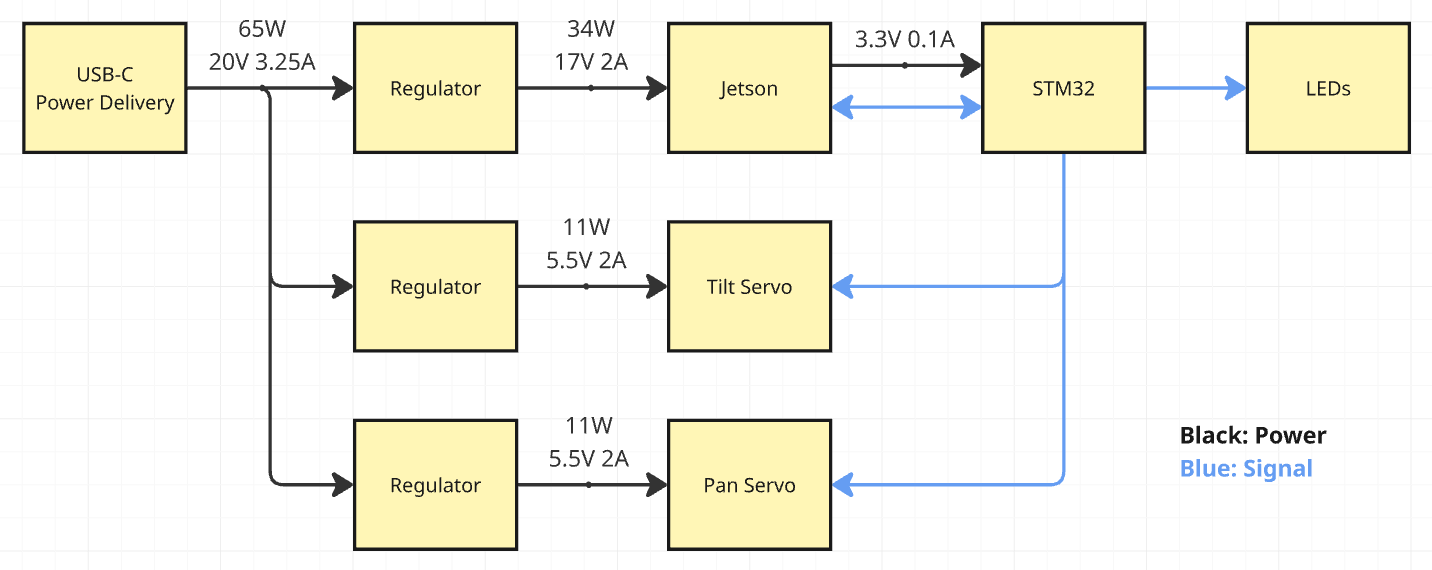
\includegraphics[width=0.95\textwidth]{block_diagram.png}
  \caption{System block diagram showing power delivery from USB-C PD
    through three independent buck converters to the Jetson (17V),
    tilt servo (5.5V), and pan servo (5.5V). The STM32F405 receives
    3.3V from the Jetson header and communicates via UART while
    generating PWM signals for servo control. Black arrows indicate
    power flow; blue arrows indicate signal flow.}
  \label{fig:block-diagram}
\end{figure}

The USB-C connector accepts 20V/3.25A from a PD-compliant source. The
HUSB237 PD controller negotiates the 20V contract with the source.
Three independent TPS54308 buck converters step down the 20V input to
the required output voltages. The STM32F405 interfaces with the Jetson
via UART (PA9/PA10) for command and telemetry exchange, and drives the
servos via software-generated PWM signals on PB5 (tilt) and PB6 (pan).

\section{Component Selection}
\label{sec:component-selection}

\subsection{Buck Converter: TPS54308}

The Texas Instruments TPS54308 was selected for all three DC-DC
converters based on the following criteria:

\begin{itemize}[leftmargin=*]
  \item \textbf{Input voltage range}: 4.5V to 28V covers the 20V PD
        input with margin for transients.
  \item \textbf{Output current}: 3A maximum continuous output exceeds
        the 2A requirements for both the Jetson and servo rails.
  \item \textbf{Package}: SOT-23-6 enables compact layout and adequate
        thermal performance for the power levels involved.
  \item \textbf{Switching frequency}: Fixed 350kHz with Forced
        Continuous Conduction Mode (FCCM) provides predictable noise
        characteristics.
  \item \textbf{Internal compensation}: Eliminates external
        compensation components, reducing BOM complexity and board area.
\end{itemize}

The TPS54308 features an internal 0.6V voltage reference ($V_{ref}$)
used in the feedback resistor divider to set the output voltage~\citep{TI_TPS54308_2021}.

\subsection{USB PD Controller: HUSB237}

The Hynetek HUSB237-AA001-DN06R USB PD sink controller was selected for
USB-C power negotiation:

\begin{itemize}[leftmargin=*]
  \item \textbf{Minimalist configuration}: A single external
        capacitor (C23 = 20nF) on the VSET pin selects the target 20V
        voltage, eliminating the need for external resistors or
        programming.
  \item \textbf{Power capability}: Supports up to 20V/5A (100W),
        exceeding the 65W requirement.
  \item \textbf{Package}: DFN-6L (2mm $\times$ 2mm) for compact layout.
\end{itemize}

The HUSB237 negotiates with the USB-C PD source to request the voltage
configured by the VSET capacitor; a 20nF capacitor selects 20V~\citep{Hynetek_HUSB237_2024}.

\subsection{Microcontroller: STM32F405RGIx}

The STMicroelectronics STM32F405RGIx was selected as mandated by SRS
constraint SC-2 (``gimbal control hardware shall use an STM32-family
microcontroller board supplied or approved by the McMaster Rocketry
Team''). Key specifications:

\begin{itemize}[leftmargin=*]
  \item \textbf{Core}: ARM Cortex-M4 with FPU at up to 168MHz
  \item \textbf{Memory}: 1MB Flash, 192KB SRAM
  \item \textbf{Peripherals}: USART, timers, GPIO, SWD debug
  \item \textbf{Package}: LQFP-64 for hand-solderability
\end{itemize}

The MCU runs the \texttt{embassy-rs} async runtime for real-time servo
control and UART communication~\citep{ST_STM32F405_2022}.

\subsection{Inductor: FXL0630-15q-M}

The Taiyo Yuden FXL0630-15q-M 15$\mu$H inductor was selected for all
three buck converters. Its 6.3mm $\times$ 6.0mm package provides
current rating suitable for the 3A TPS54308 application. The 15$\mu$H
value balances ripple current and physical size at the 350kHz
switching frequency.

\subsection{Connectors}

\begin{itemize}[leftmargin=*]
  \item \textbf{Jetson interface}: Samtec ESQ-106-33-L-D 6-pin header
        carries UART (RX/TX), 3.3V, and ground between the PCB and
        Jetson expansion header.
  \item \textbf{Servo outputs}: 3-pin 0.1" headers (signal, power,
        ground) for standard hobby servo connectors.
  \item \textbf{Jetson power}: 2-pin screw terminal for the 17V output
        to the Jetson's DC barrel jack.
  \item \textbf{USB-C}: HX TYPE-C 16P SMD 5A connector for PD input.
  \item \textbf{Debug}: SWD header for programming and debugging the
        STM32F405.
\end{itemize}

\section{Circuit Design and Calculations}
\label{sec:circuit-design}

This section details the circuit implementation for each functional
block, including component value calculations.

\subsection{USB-C Power Delivery}
\label{subsec:usb-pd}

The USB-C power input stage uses the HUSB237 PD controller to negotiate
20V from the connected power source. Figure~\ref{fig:schematic-4}
shows the implementation.

\begin{figure}[H]
  \centering
  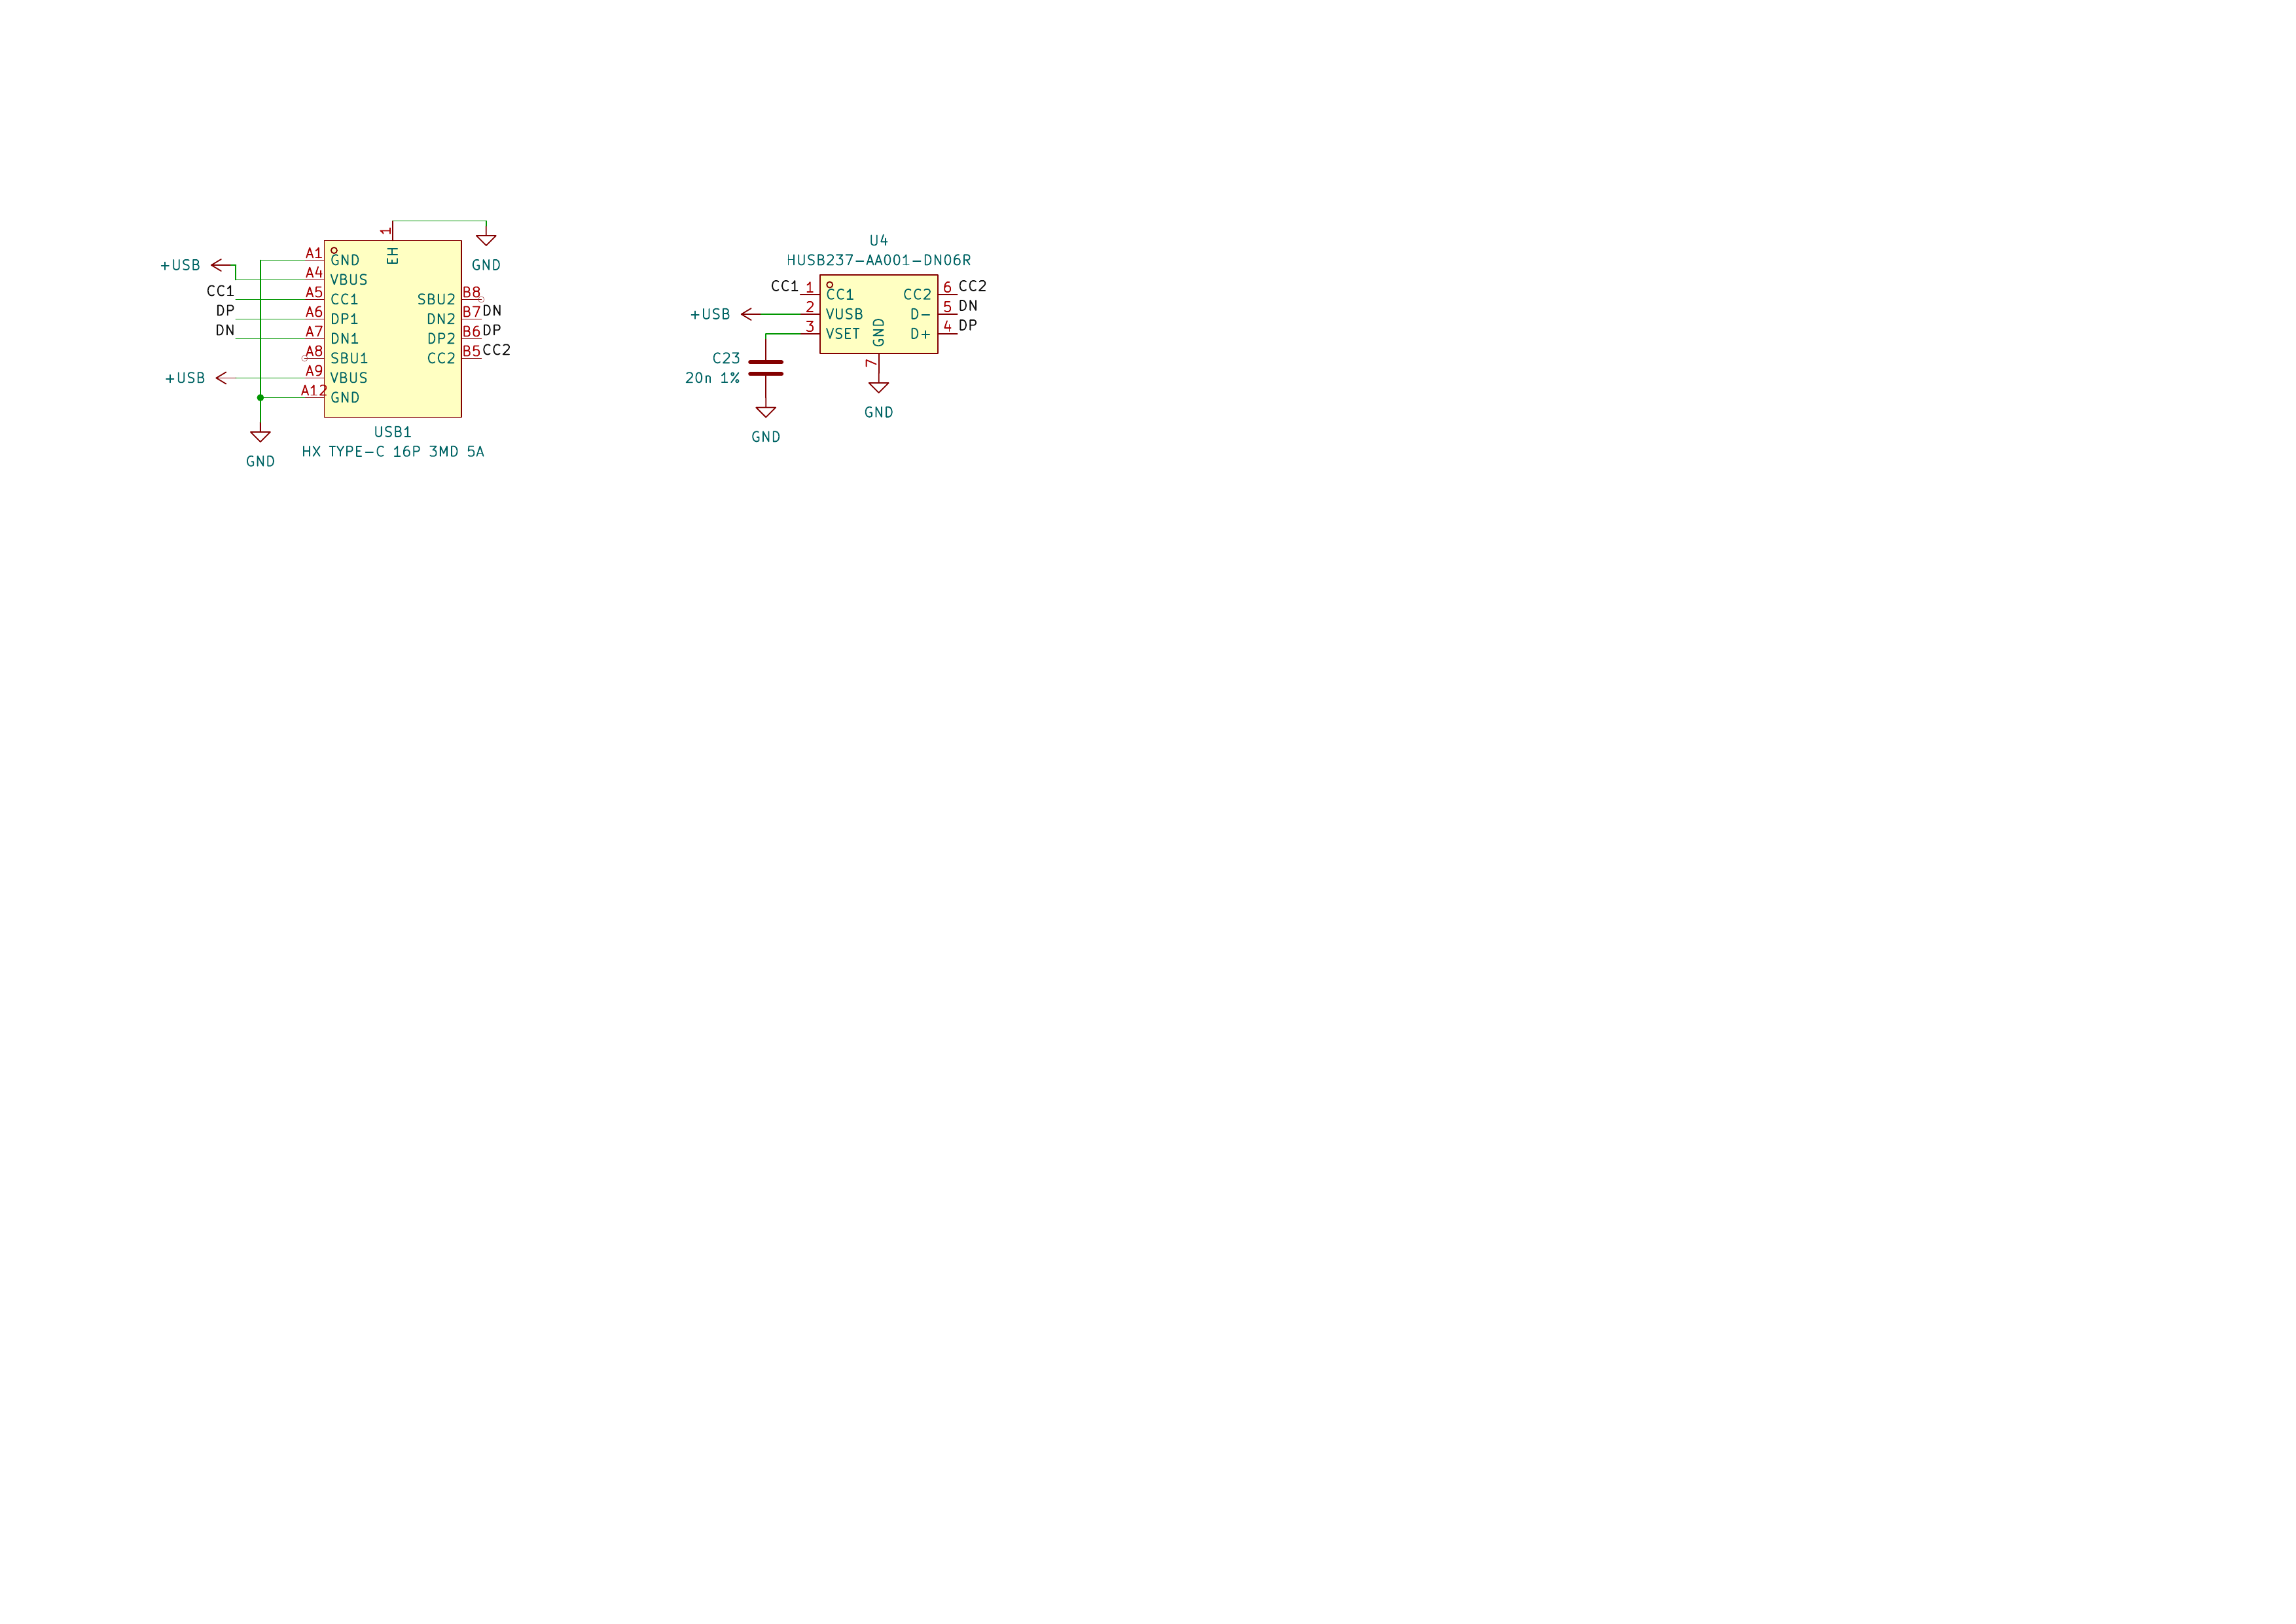
\includegraphics[width=0.85\textwidth]{schematics-4.png}
  \caption{USB-C connector and HUSB237 PD controller schematic.
    The HUSB237 (U4) negotiates the PD contract; capacitor C23 (20nF)
    on VSET selects 20V target. USB1 is the Type-C receptacle.}
  \label{fig:schematic-4}
\end{figure}

The HUSB237 VSET pin uses an external capacitor to configure the target
RDO (Request Data Object) voltage. The relationship between capacitance
and target voltage is defined by the manufacturer; for the HUSB237,
a 20nF capacitor selects 20V. This simple configuration eliminates the
need for external resistors or I2C programming.

Decoupling capacitor C23 (20nF, 1\% tolerance ceramic) connects between
VSET and ground. A 1$\mu$F decoupling capacitor near the VBUS pin
provides supply filtering. The CC1 and CC2 pins connect to the USB-C
Configuration Channel lines for PD communication.

\subsection{Servo Power Regulators}
\label{subsec:servo-regulators}

Two identical TPS54308 buck converters generate the 5.5V rails for the
pan and tilt servos. Figure~\ref{fig:schematic-2} shows one channel;
the second channel is duplicated.

\begin{figure}[H]
  \centering
  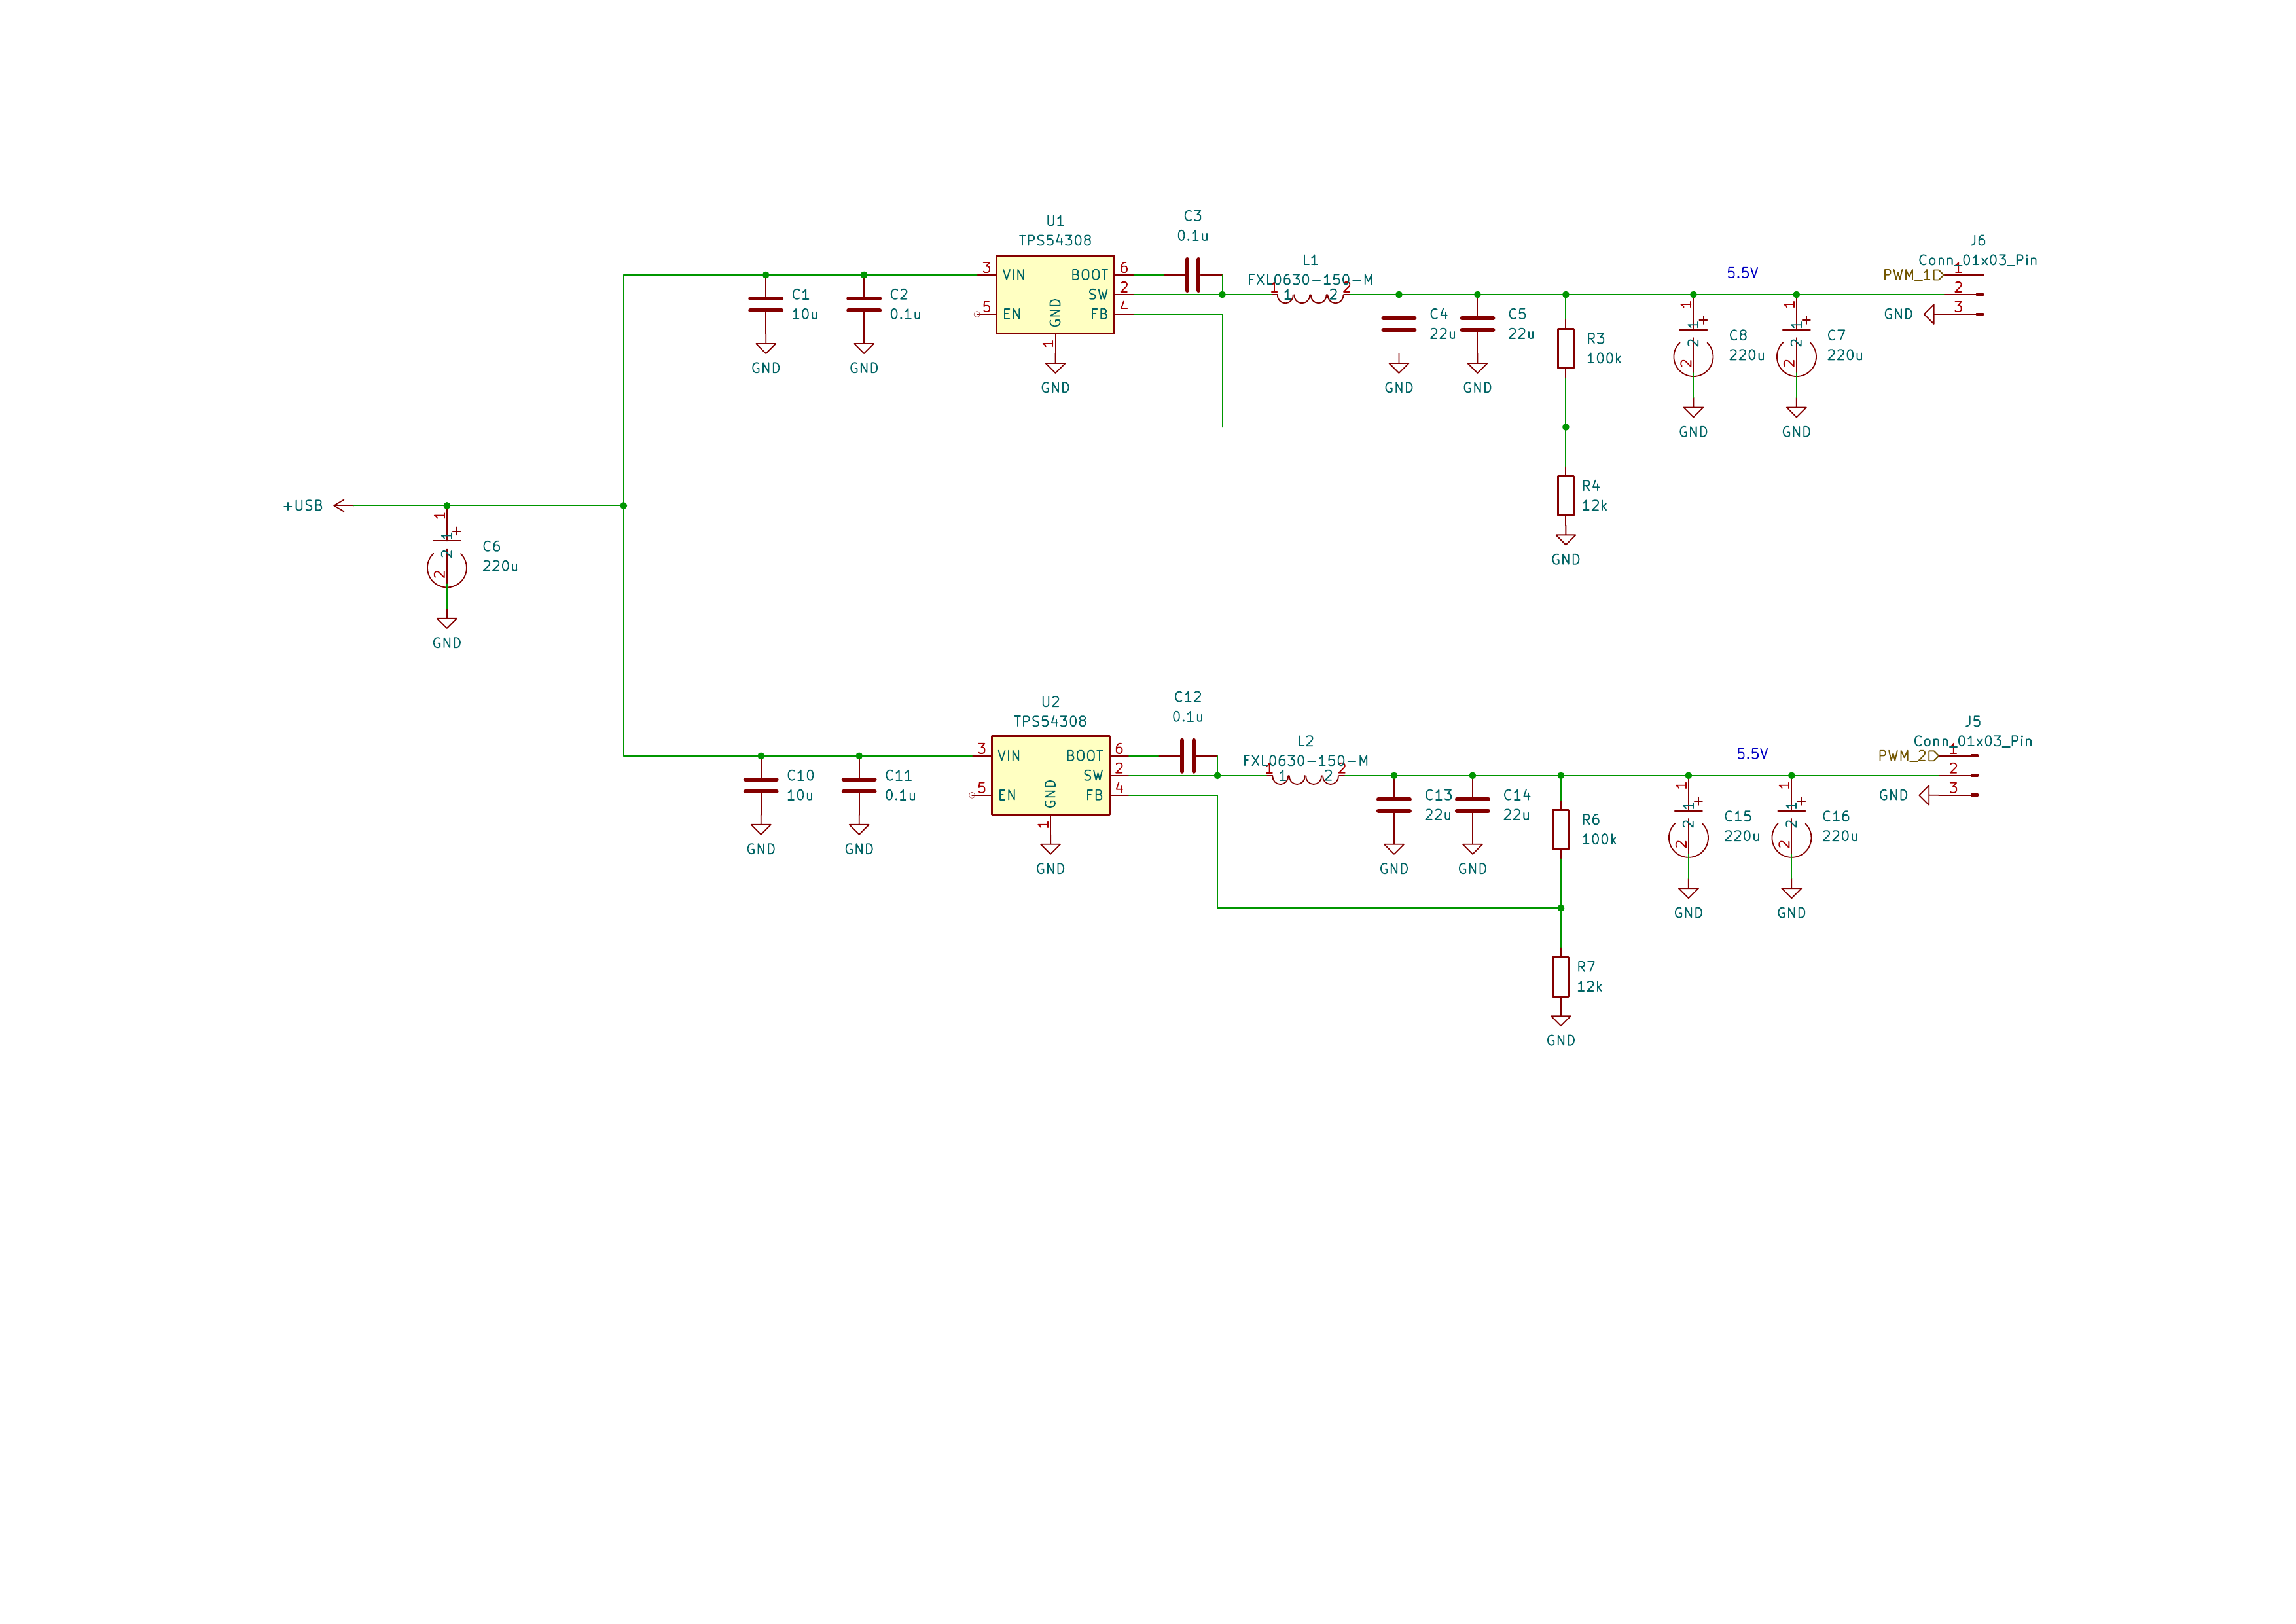
\includegraphics[width=0.95\textwidth]{schematics-2.png}
  \caption{Servo power regulator schematic (one channel shown; two
    identical channels implemented). The TPS54308 (U2) steps down 20V
    to 5.5V with feedback divider R3/R4 and output filter capacitors
    C8, C7, C13, C14, C5.}
  \label{fig:schematic-2}
\end{figure}

\subsubsection{Output Voltage Calculation}

The TPS54308 regulates its output to maintain 0.6V at the FB (feedback)
pin. The output voltage is set by a resistive divider:

\begin{equation}
  V_{out} = V_{ref} \times \left(1 + \frac{R_{top}}{R_{bottom}}\right)
\end{equation}

where $V_{ref} = 0.6$V (internal reference).

For the servo rail ($V_{out} \approx 5.5$V):
\begin{align}
  R_{top} &= R_3 = 100\text{k}\Omega \\
  R_{bottom} &= R_4 = 12\text{k}\Omega \\
  V_{out} &= 0.6 \times \left(1 + \frac{100\text{k}}{12\text{k}}\right) \\
          &= 0.6 \times (1 + 8.333) \\
          &= 0.6 \times 9.333 \\
          &= 5.6\text{V} \approx 5.5\text{V (nominal)}
\end{align}

The 5.6V output provides margin above the nominal 5.5V to compensate
for cable drops while remaining below the typical 6V maximum rating
of hobby servos.

\subsubsection{Component Selection}

\begin{itemize}[leftmargin=*]
  \item \textbf{Inductor}: L1 (FXL0630-15q-M, 15$\mu$H) selected
        for 350kHz operation at 2A load.
  \item \textbf{Output capacitors}: C8/C7 (220$\mu$F electrolytic)
        provide bulk capacitance for transient servo loads; C13/C14
        (22$\mu$F ceramic) filter high-frequency ripple.
  \item \textbf{Input capacitors}: C1 (10$\mu$F) and C2 (0.1$\mu$F)
        provide input filtering.
  \item \textbf{Boot capacitor}: C3 (0.1$\mu$F) between BOOT and SW
        pins provides gate drive voltage for the high-side MOSFET.
\end{itemize}

\subsection{Jetson Power Regulator}
\label{subsec:jetson-regulator}

A third TPS54308 buck converter generates the 17V rail for the Jetson
Orin Nano. Figure~\ref{fig:schematic-3} shows the circuit.

\begin{figure}[H]
  \centering
  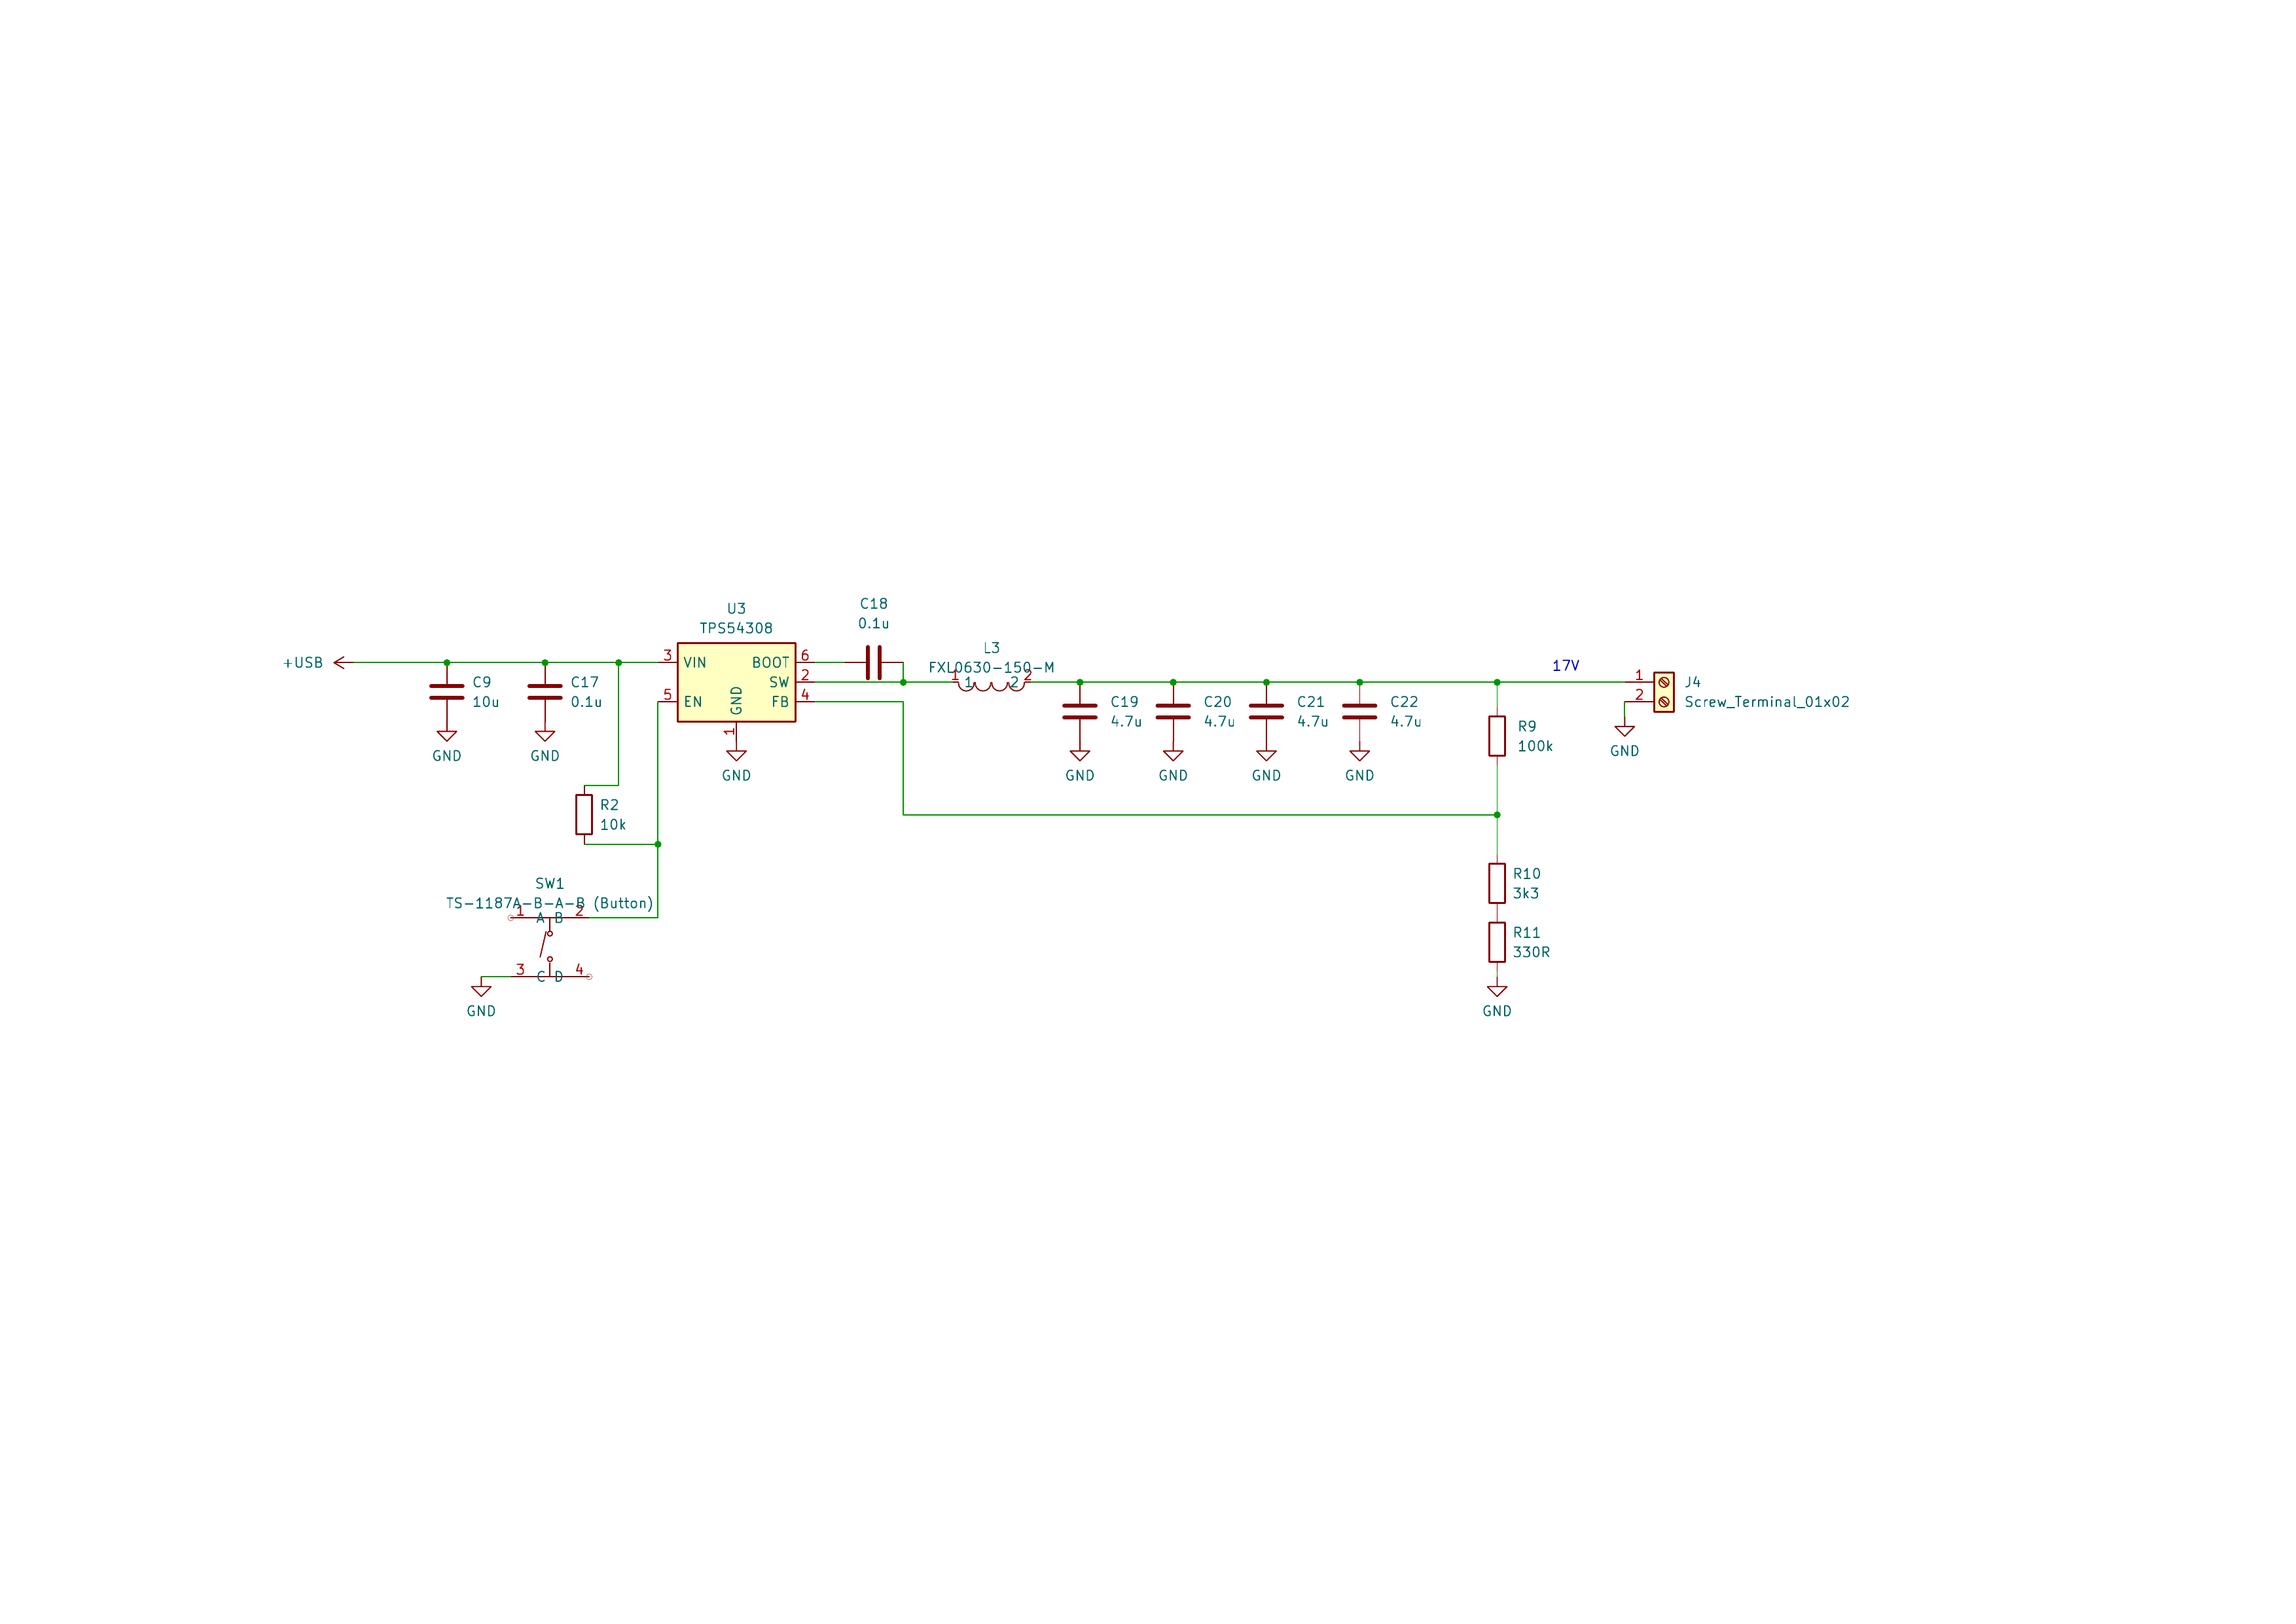
\includegraphics[width=0.95\textwidth]{schematics-3.png}
  \caption{Jetson power regulator schematic. The TPS54308 (U3) steps
    down 20V to 17V with feedback divider R9/R10/R11. The EN pin is
    controlled by switch SW1 for power control. Output filtering uses
    four 4.7$\mu$F ceramic capacitors (C19-C22).}
  \label{fig:schematic-3}
\end{figure}

\subsubsection{Output Voltage Calculation}

The feedback divider uses a series combination for $R_{bottom}$ to
achieve a non-standard ratio:

\begin{align}
  R_{top} &= R_9 = 100\text{k}\Omega \\
  R_{bottom} &= R_{10} + R_{11} = 3.3\text{k}\Omega + 330\Omega = 3.63\text{k}\Omega \\
  V_{out} &= 0.6 \times \left(1 + \frac{100\text{k}}{3.63\text{k}}\right) \\
          &= 0.6 \times (1 + 27.55) \\
          &= 0.6 \times 28.55 \\
          &= 17.13\text{V} \approx 17\text{V (nominal)}
\end{align}

The 17V output provides margin above the Jetson's minimum 7V input
while remaining well below the maximum 20V rating~\citep{Nvidia_JetsonOrinNano_Power_2024}.

\subsubsection{Enable Circuit}

The TPS54308 EN (enable) pin controls regulator operation. Switch SW1
(TS-1187A-B-A-B tactile button) pulls the EN pin high when pressed,
activating the regulator. This provides a soft-start capability for
the Jetson power rail.

\subsection{STM32 Microcontroller}
\label{subsec:stm32}

The STM32F405RGIx microcontroller forms the core of the gimbal
control system. Figure~\ref{fig:schematic-1} shows the MCU and its
supporting circuitry.

\begin{figure}[H]
  \centering
  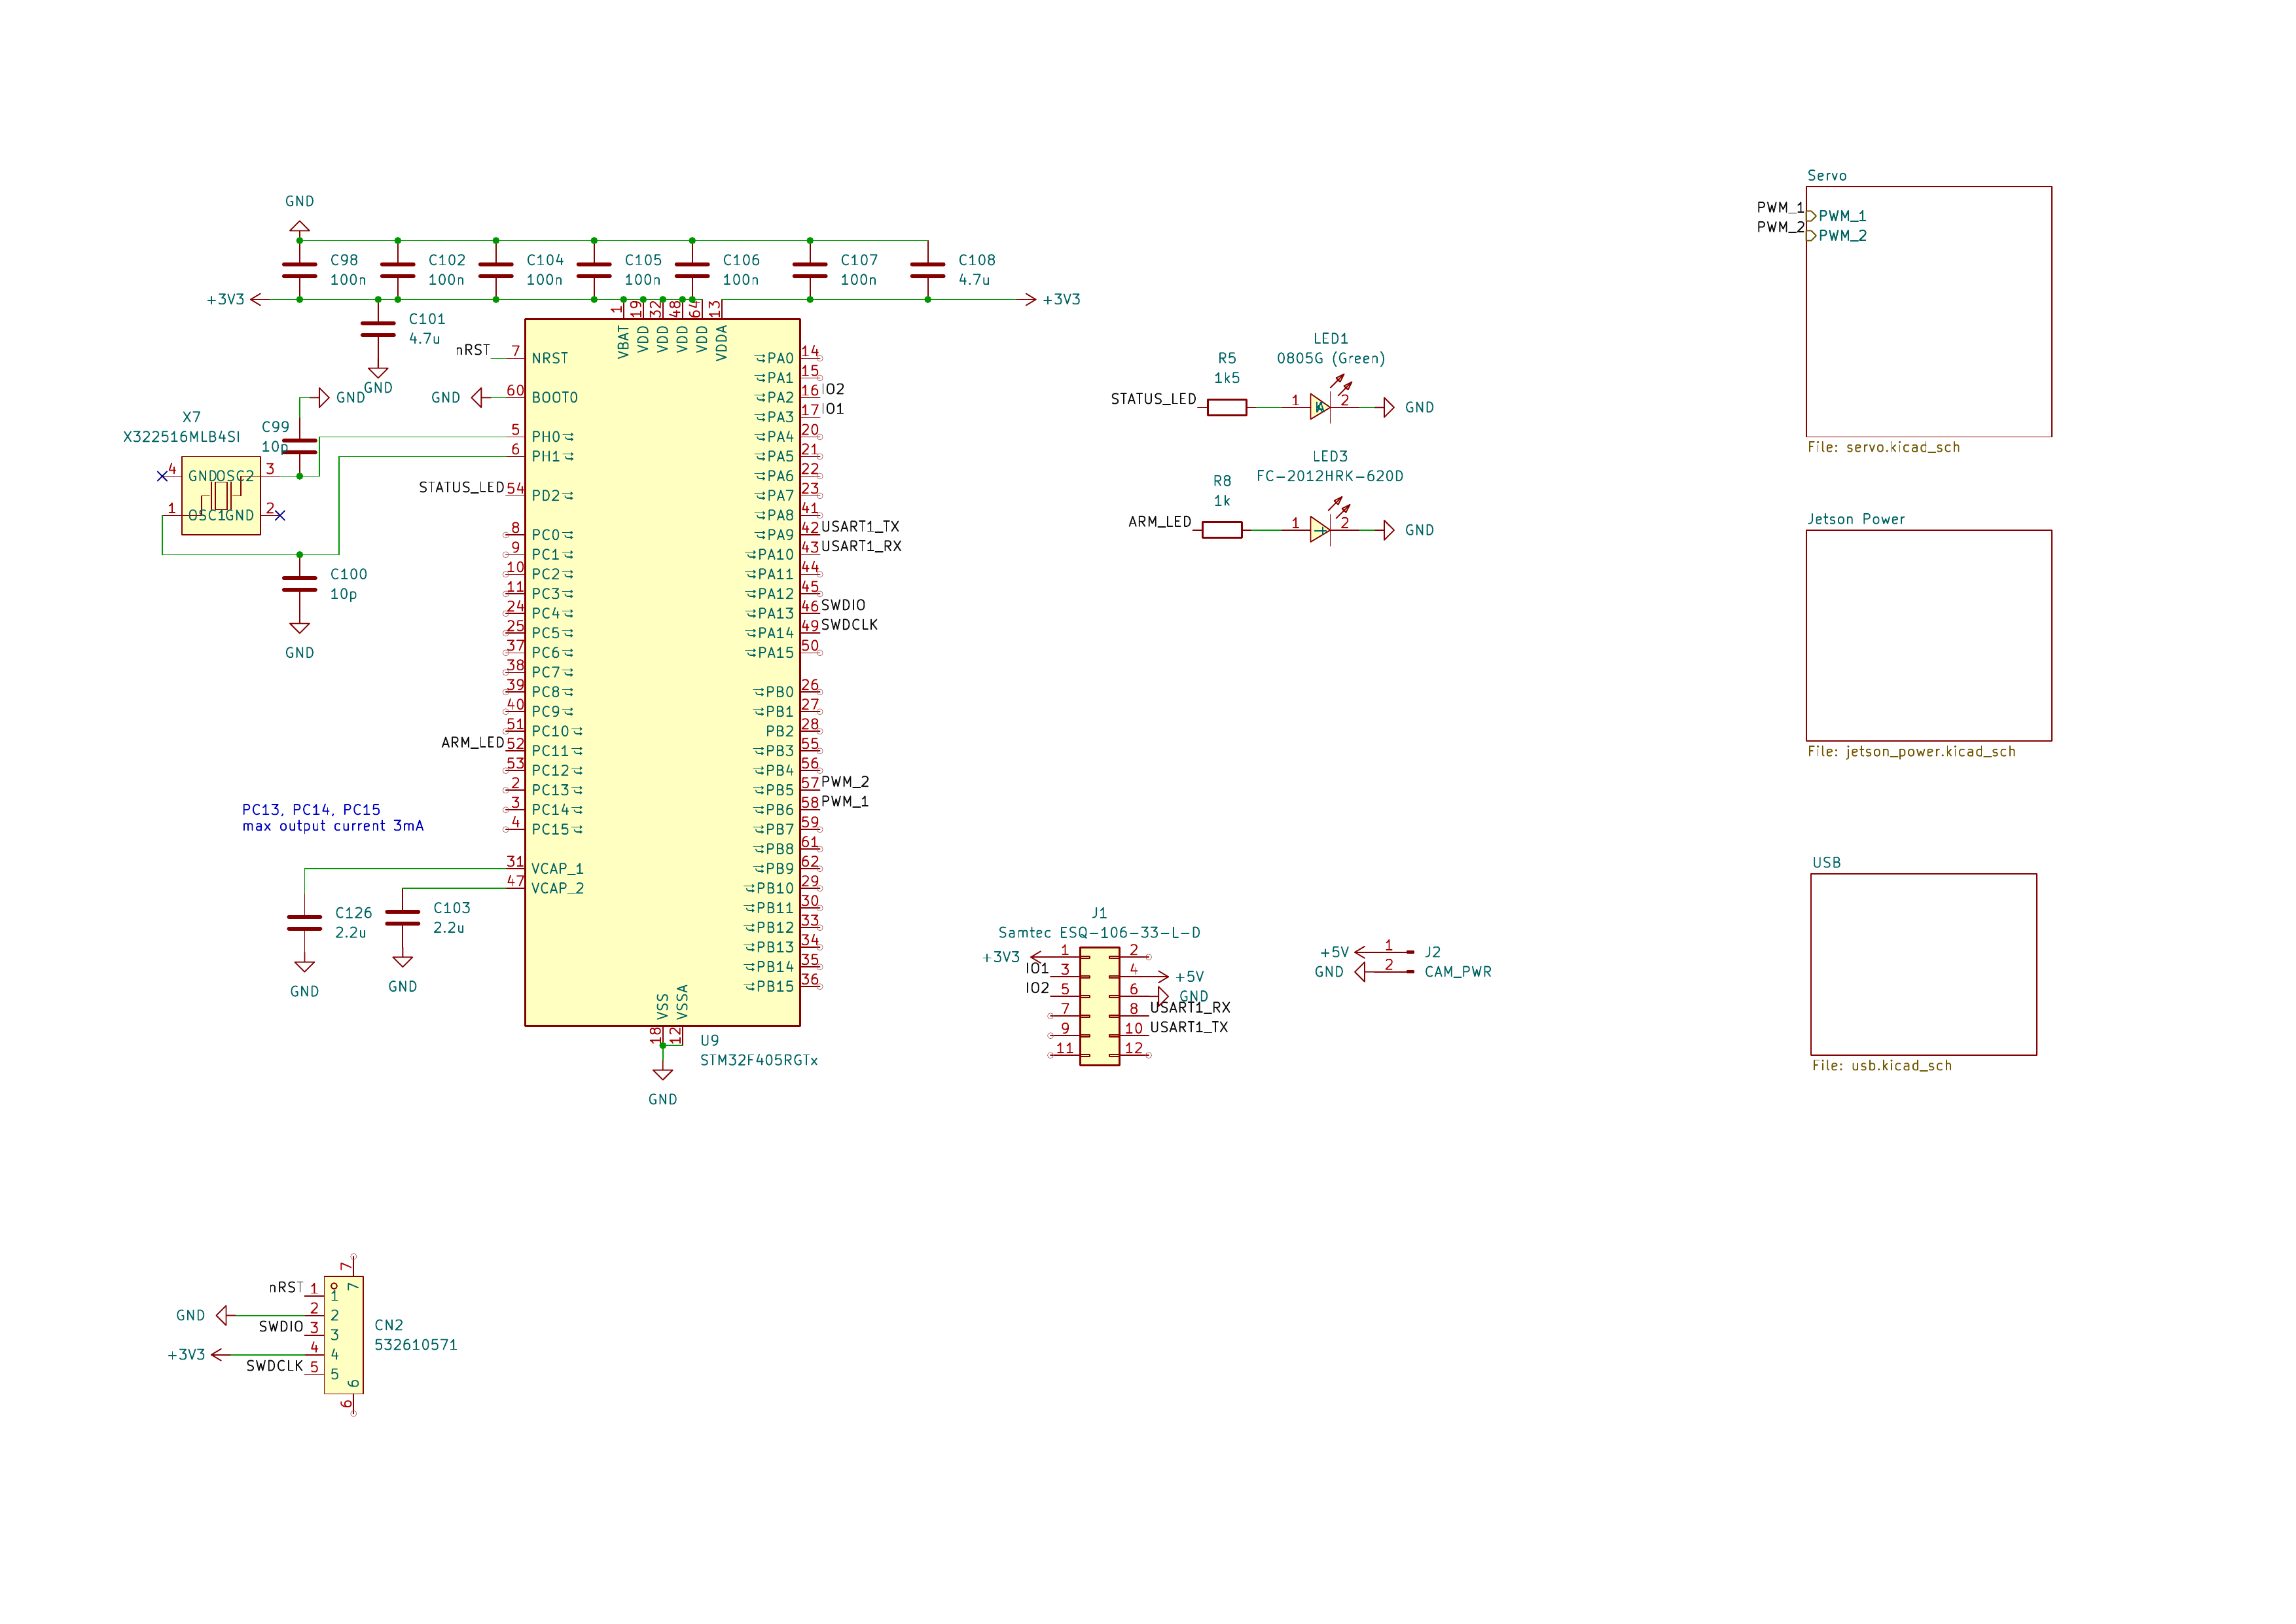
\includegraphics[width=0.95\textwidth]{schematics-1.png}
  \caption{STM32F405 microcontroller schematic. The MCU (U9) includes
    decoupling capacitors (C98-C108), VCAP capacitors (C126, C103),
    8MHz crystal (X7) with load capacitors, status LEDs, and the
    Samtec connector for Jetson interface.}
  \label{fig:schematic-1}
\end{figure}

\subsubsection{Decoupling and Power}

The STM32F405 requires extensive decoupling for stable operation:

\begin{itemize}[leftmargin=*]
  \item \textbf{VDD decoupling}: Five 100nF ceramic capacitors (C98,
        C102, C104, C105, C106) distributed near the VDD pins filter
        high-frequency noise.
  \item \textbf{Bulk decoupling}: One 4.7$\mu$F capacitor (C101)
        provides low-frequency energy storage.
  \item \textbf{VCAP capacitors}: Two 2.2$\mu$F capacitors (C126,
        C103) connect to the VCAP\_1 and VCAP\_2 pins for the internal
        voltage regulator.
\end{itemize}

\subsubsection{Clock Source}

An 8MHz crystal (X7, X322516MLB4SI) with 10pF load capacitors (C99,
C100) provides the HSE (High-Speed External) clock. The internal PLL
multiplies this to the system clock frequency (up to 168MHz).

\subsubsection{Status Indicators}

Two LEDs provide visual status indication:

\begin{itemize}[leftmargin=*]
  \item \textbf{STATUS\_LED} (green, D1): Controlled via PD2; indicates
        system status/heartbeat.
  \item \textbf{ARM\_LED} (red/amber, D3): Controlled via PC11;
        indicates armed/disarmed state.
\end{itemize}

Current-limiting resistors R5 (1k$\Omega$) and R8 (1k$\Omega$) set LED
current to approximately 3mA.

\subsection{Communication Interfaces}
\label{subsec:communication}

The PCB implements two primary communication interfaces between the
STM32 and external systems.

\subsubsection{UART to Jetson}

USART1 on the STM32F405 provides the serial link to the Jetson Orin
Nano:

\begin{itemize}[leftmargin=*]
  \item \textbf{Pins}: PA9 (USART1\_TX), PA10 (USART1\_RX)
  \item \textbf{Configuration}: 115200 baud, 8 data bits, no parity,
        1 stop bit (8N1)
  \item \textbf{Protocol}: Gimbal Protocol as defined by McMaster
        Rocketry Team (command IDs 0x00--0x07)
  \item \textbf{Connector}: Samtec ESQ-106-33-L-D (J1) carries TX, RX,
        3.3V, and GND
\end{itemize}

\subsubsection{PWM to Servos}

Software-generated PWM signals control the servos:

\begin{itemize}[leftmargin=*]
  \item \textbf{Tilt servo}: PB5, 50Hz update, 1040--2360$\mu$s pulse
        width, -90\degree to +90\degree range, reversed direction,
        49\degree offset.
  \item \textbf{Pan servo}: PB6, 50Hz update, 1040--2360$\mu$s pulse
        width, -90\degree to +90\degree range, standard direction,
        -7\degree offset.
\end{itemize}

The pulse width is calculated as:
\begin{equation}
  \text{pulse\_width} = 1040 + \frac{\text{angle} + 90}{180} \times 1320 \quad \mu\text{s}
\end{equation}

\section{PCB Layout}
\label{sec:layout}

Figure~\ref{fig:layout} shows the PCB layout for the ``Tracking Cam
Prototype 0.5'' board.

\begin{figure}[H]
  \centering
  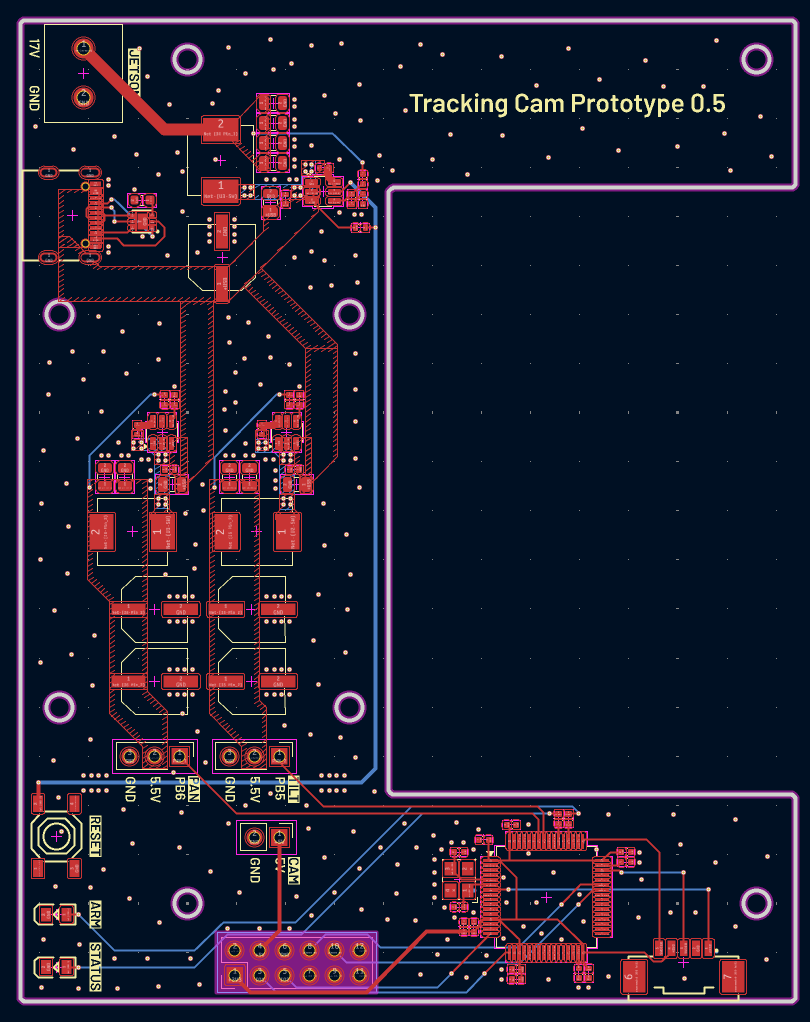
\includegraphics[width=0.95\textwidth]{layout.png}
  \caption{PCB layout of the Tracking Cam Prototype 0.5. The board
    measures approximately 100mm $\times$ 80mm. Power converters are
    arranged in the upper left; the STM32 MCU is in the lower right;
    connectors are placed along the edges for accessibility. The large
    empty area accommodates mechanical mounting features and a future
    E-stop switch.}
  \label{fig:layout}
\end{figure}

\subsection{Layout Considerations}

\begin{itemize}[leftmargin=*]
  \item \textbf{Power traces}: High-current paths (20V input, 17V
        output, 5.5V outputs) use wide traces with thermal relief for
        component pads.
  \item \textbf{Ground plane}: A solid ground plane on the bottom layer
        provides low-impedance return paths and EMI reduction.
  \item \textbf{Decoupling placement}: Capacitors placed close to IC
        power pins minimize loop inductance.
  \item \textbf{Switching noise}: The TPS54308 switch node (SW) traces
        are kept short to reduce radiated EMI.
  \item \textbf{Connector placement}: USB-C, servo headers, and Jetson
        interface placed on board edges for cable management.
  \item \textbf{Mounting holes}: Four mounting holes with copper
        keepouts for mechanical attachment to the gimbal frame.
\end{itemize}

\section{Conclusion}
\label{sec:conclusion}

The ``Tracking Cam Prototype 0.5'' PCB successfully integrates the
power and control functions required for the \progname{} gimbal
tracking system. The design delivers:

\begin{itemize}[leftmargin=*]
  \item \textbf{65W USB-C PD input} with 20V negotiation via the
        HUSB237 controller.
  \item \textbf{Three regulated rails}: 17V/2A (Jetson), 5.5V/2A
        (pan servo), 5.5V/2A (tilt servo).
  \item \textbf{STM32F405-based control} with UART to Jetson and PWM
        servo outputs.
  \item \textbf{Compliance with project requirements}: STM32-family
        MCU (SRS SC-2), Jetson Orin Nano support (SRS SC-3), and
        operating temperature range 0--45\degree C (SRS EPE-1).
\end{itemize}

All feedback resistor values have been calculated and verified against
the TPS54308 0.6V reference voltage. The board is ready for assembly
and integration testing with the \progname{} system.

\bibliographystyle{plainnat}

\bibliography{../../../refs/References}

\newpage

\appendix

\section{Full Schematics}
\label{app:schematics}

This appendix presents the complete schematic set for the Tracking
Cam Prototype 0.5 PCB.

\begin{figure}[H]
  \centering
  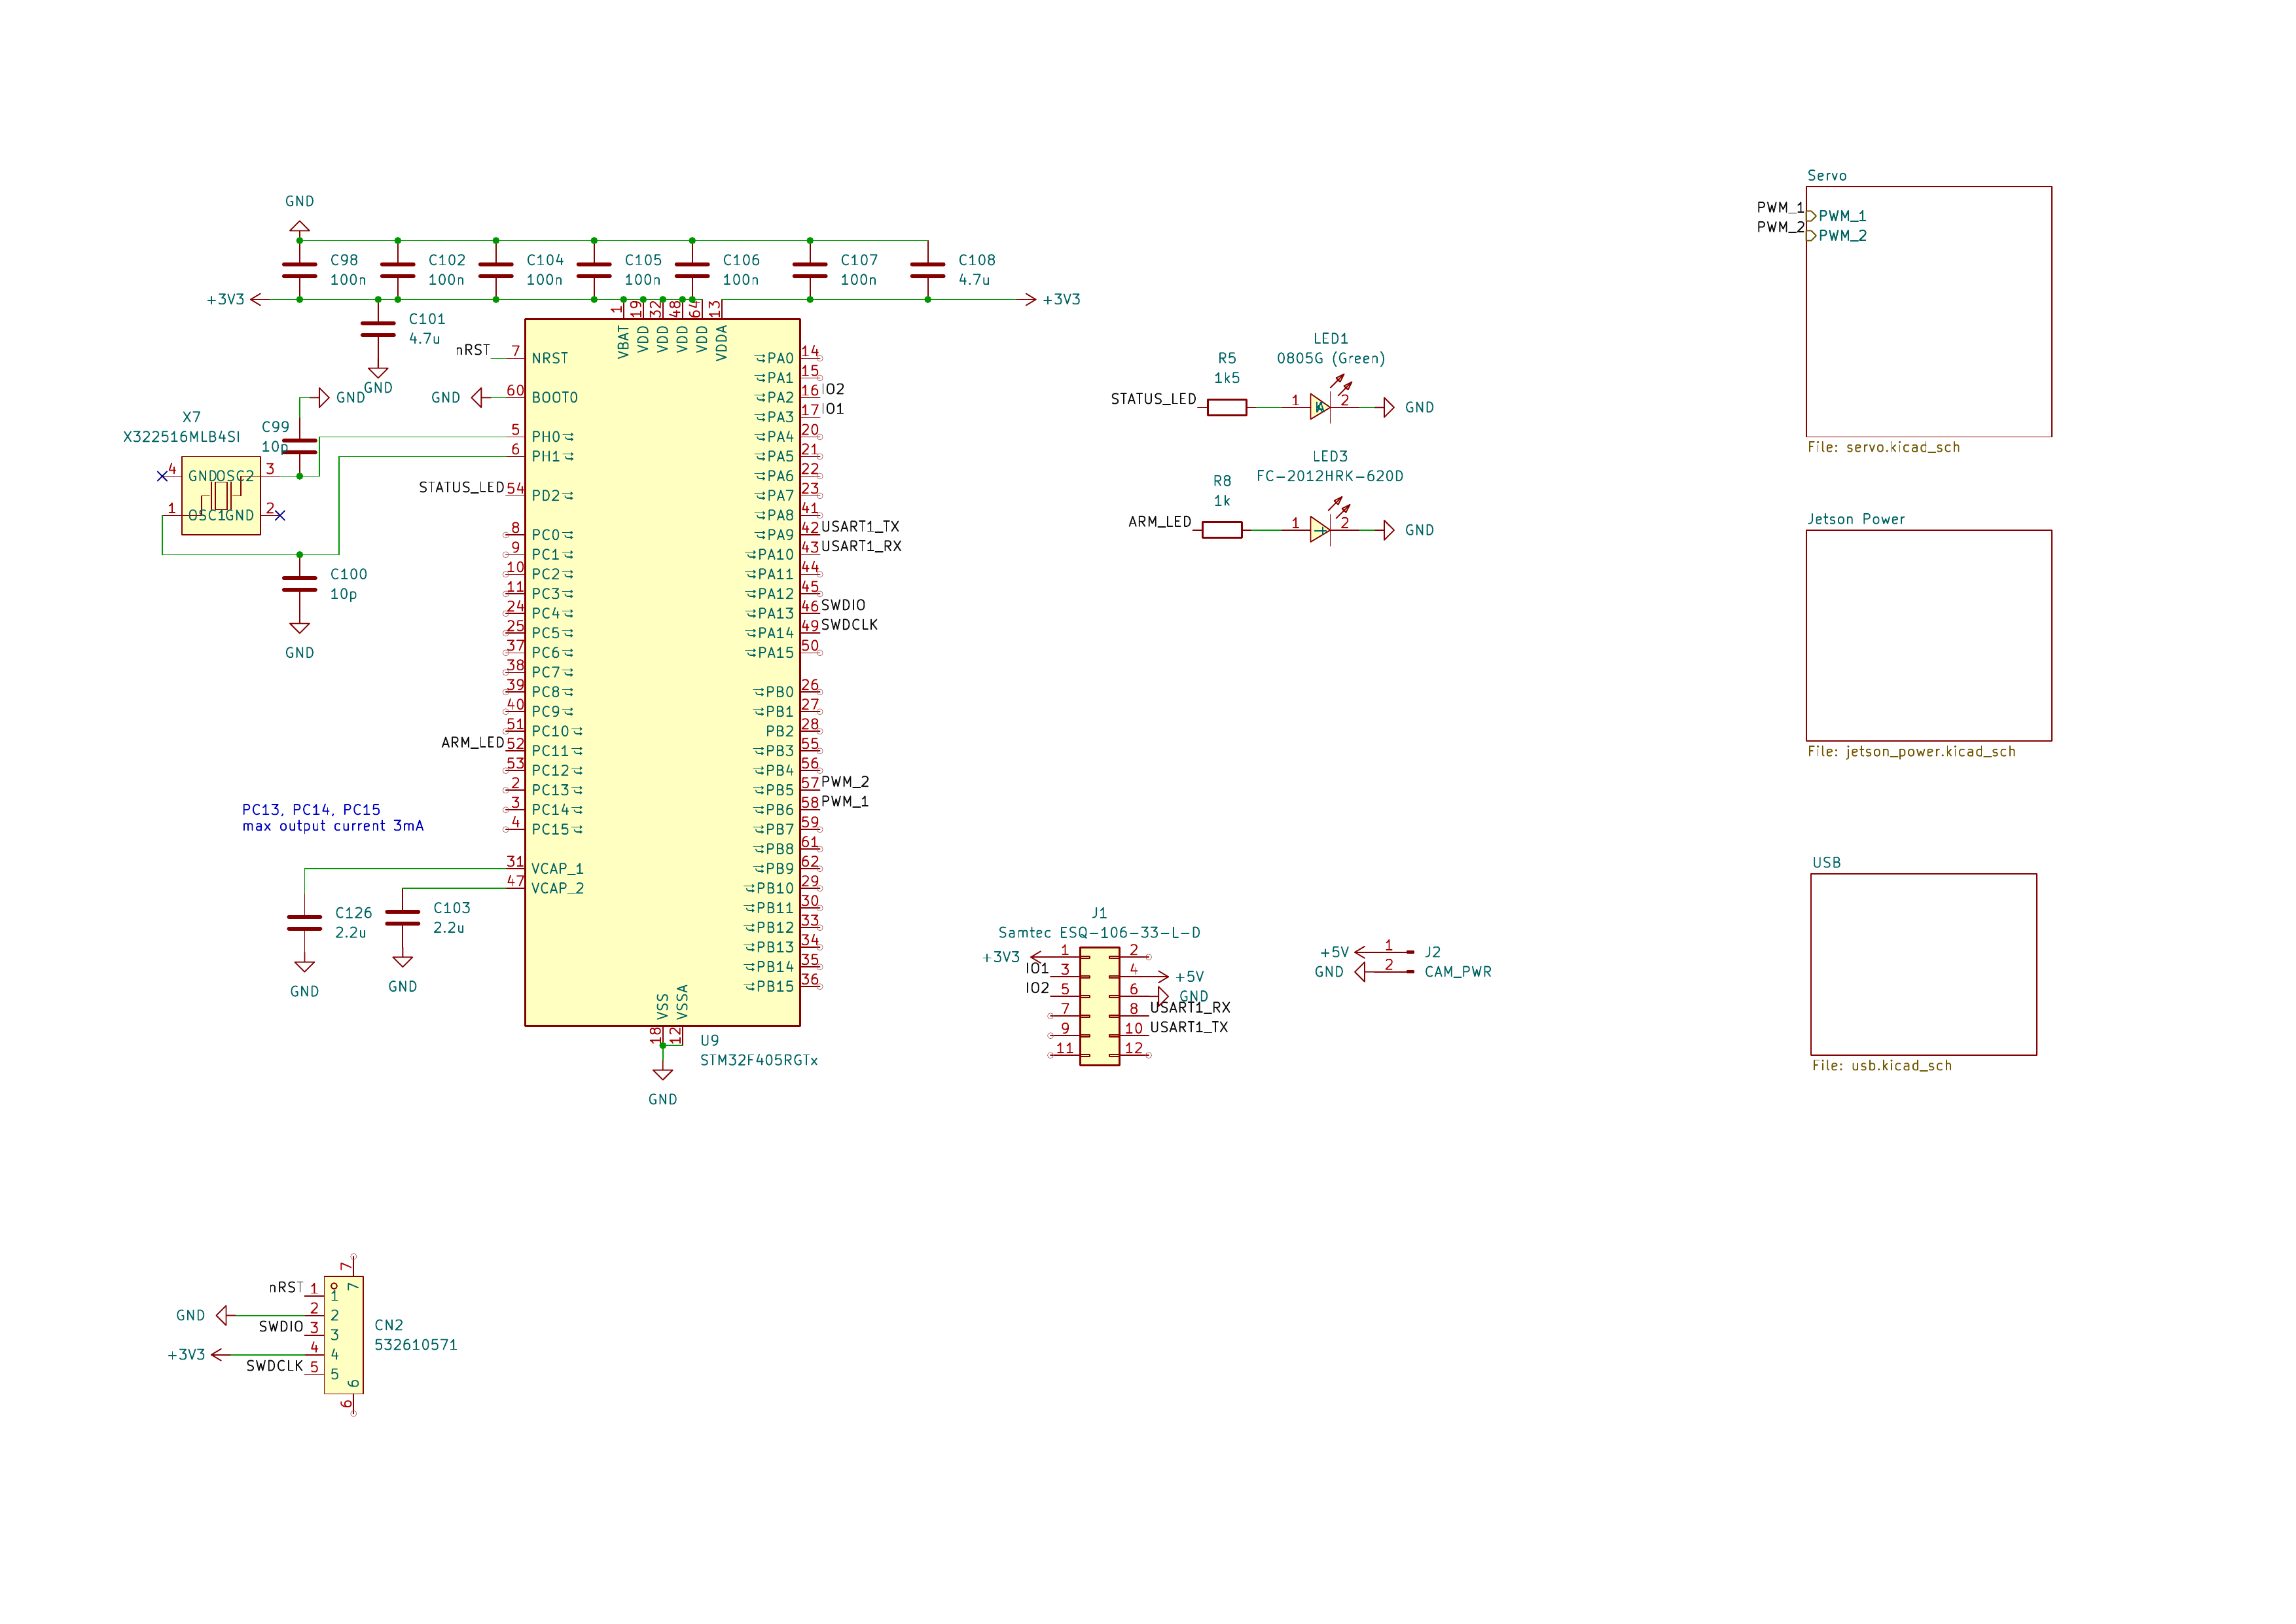
\includegraphics[width=0.95\textwidth]{schematics-1.png}
  \caption{STM32F405 microcontroller and LED schematic (Sheet 1 of 4).}
  \label{fig:schematic-full-1}
\end{figure}

\begin{figure}[H]
  \centering
  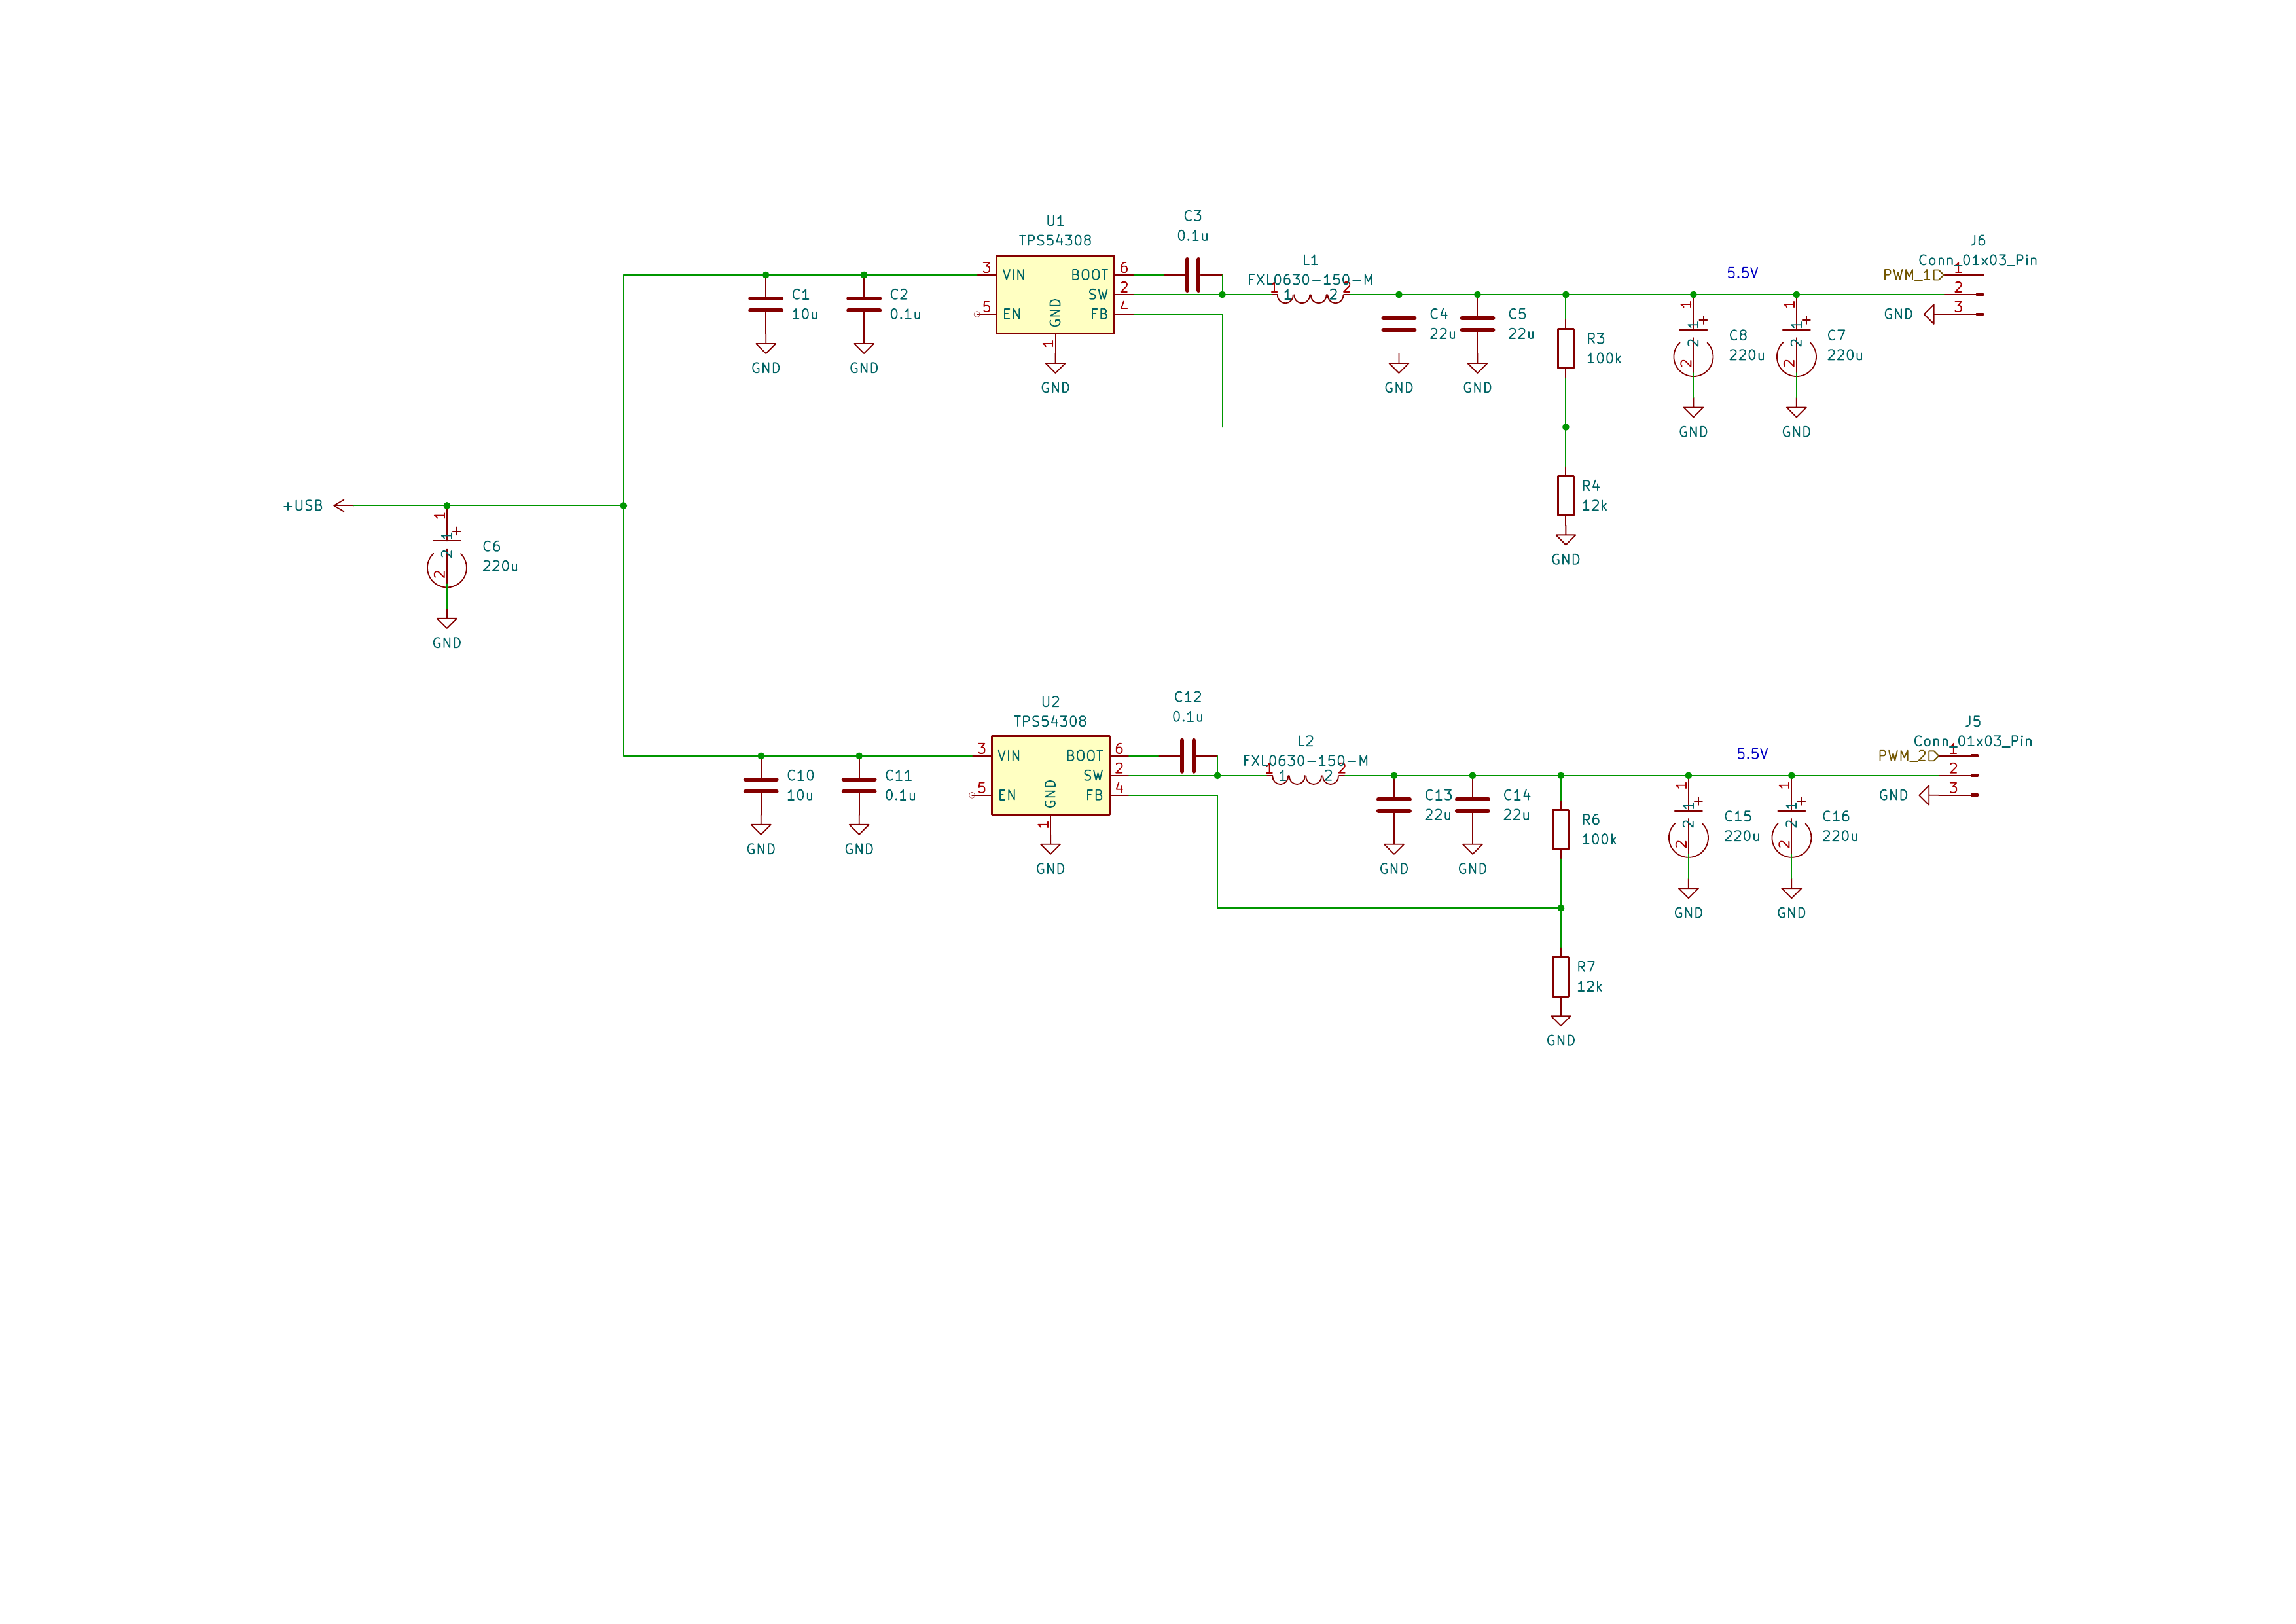
\includegraphics[width=0.95\textwidth]{schematics-2.png}
  \caption{Servo power regulators schematic (Sheet 2 of 4).}
  \label{fig:schematic-full-2}
\end{figure}

\begin{figure}[H]
  \centering
  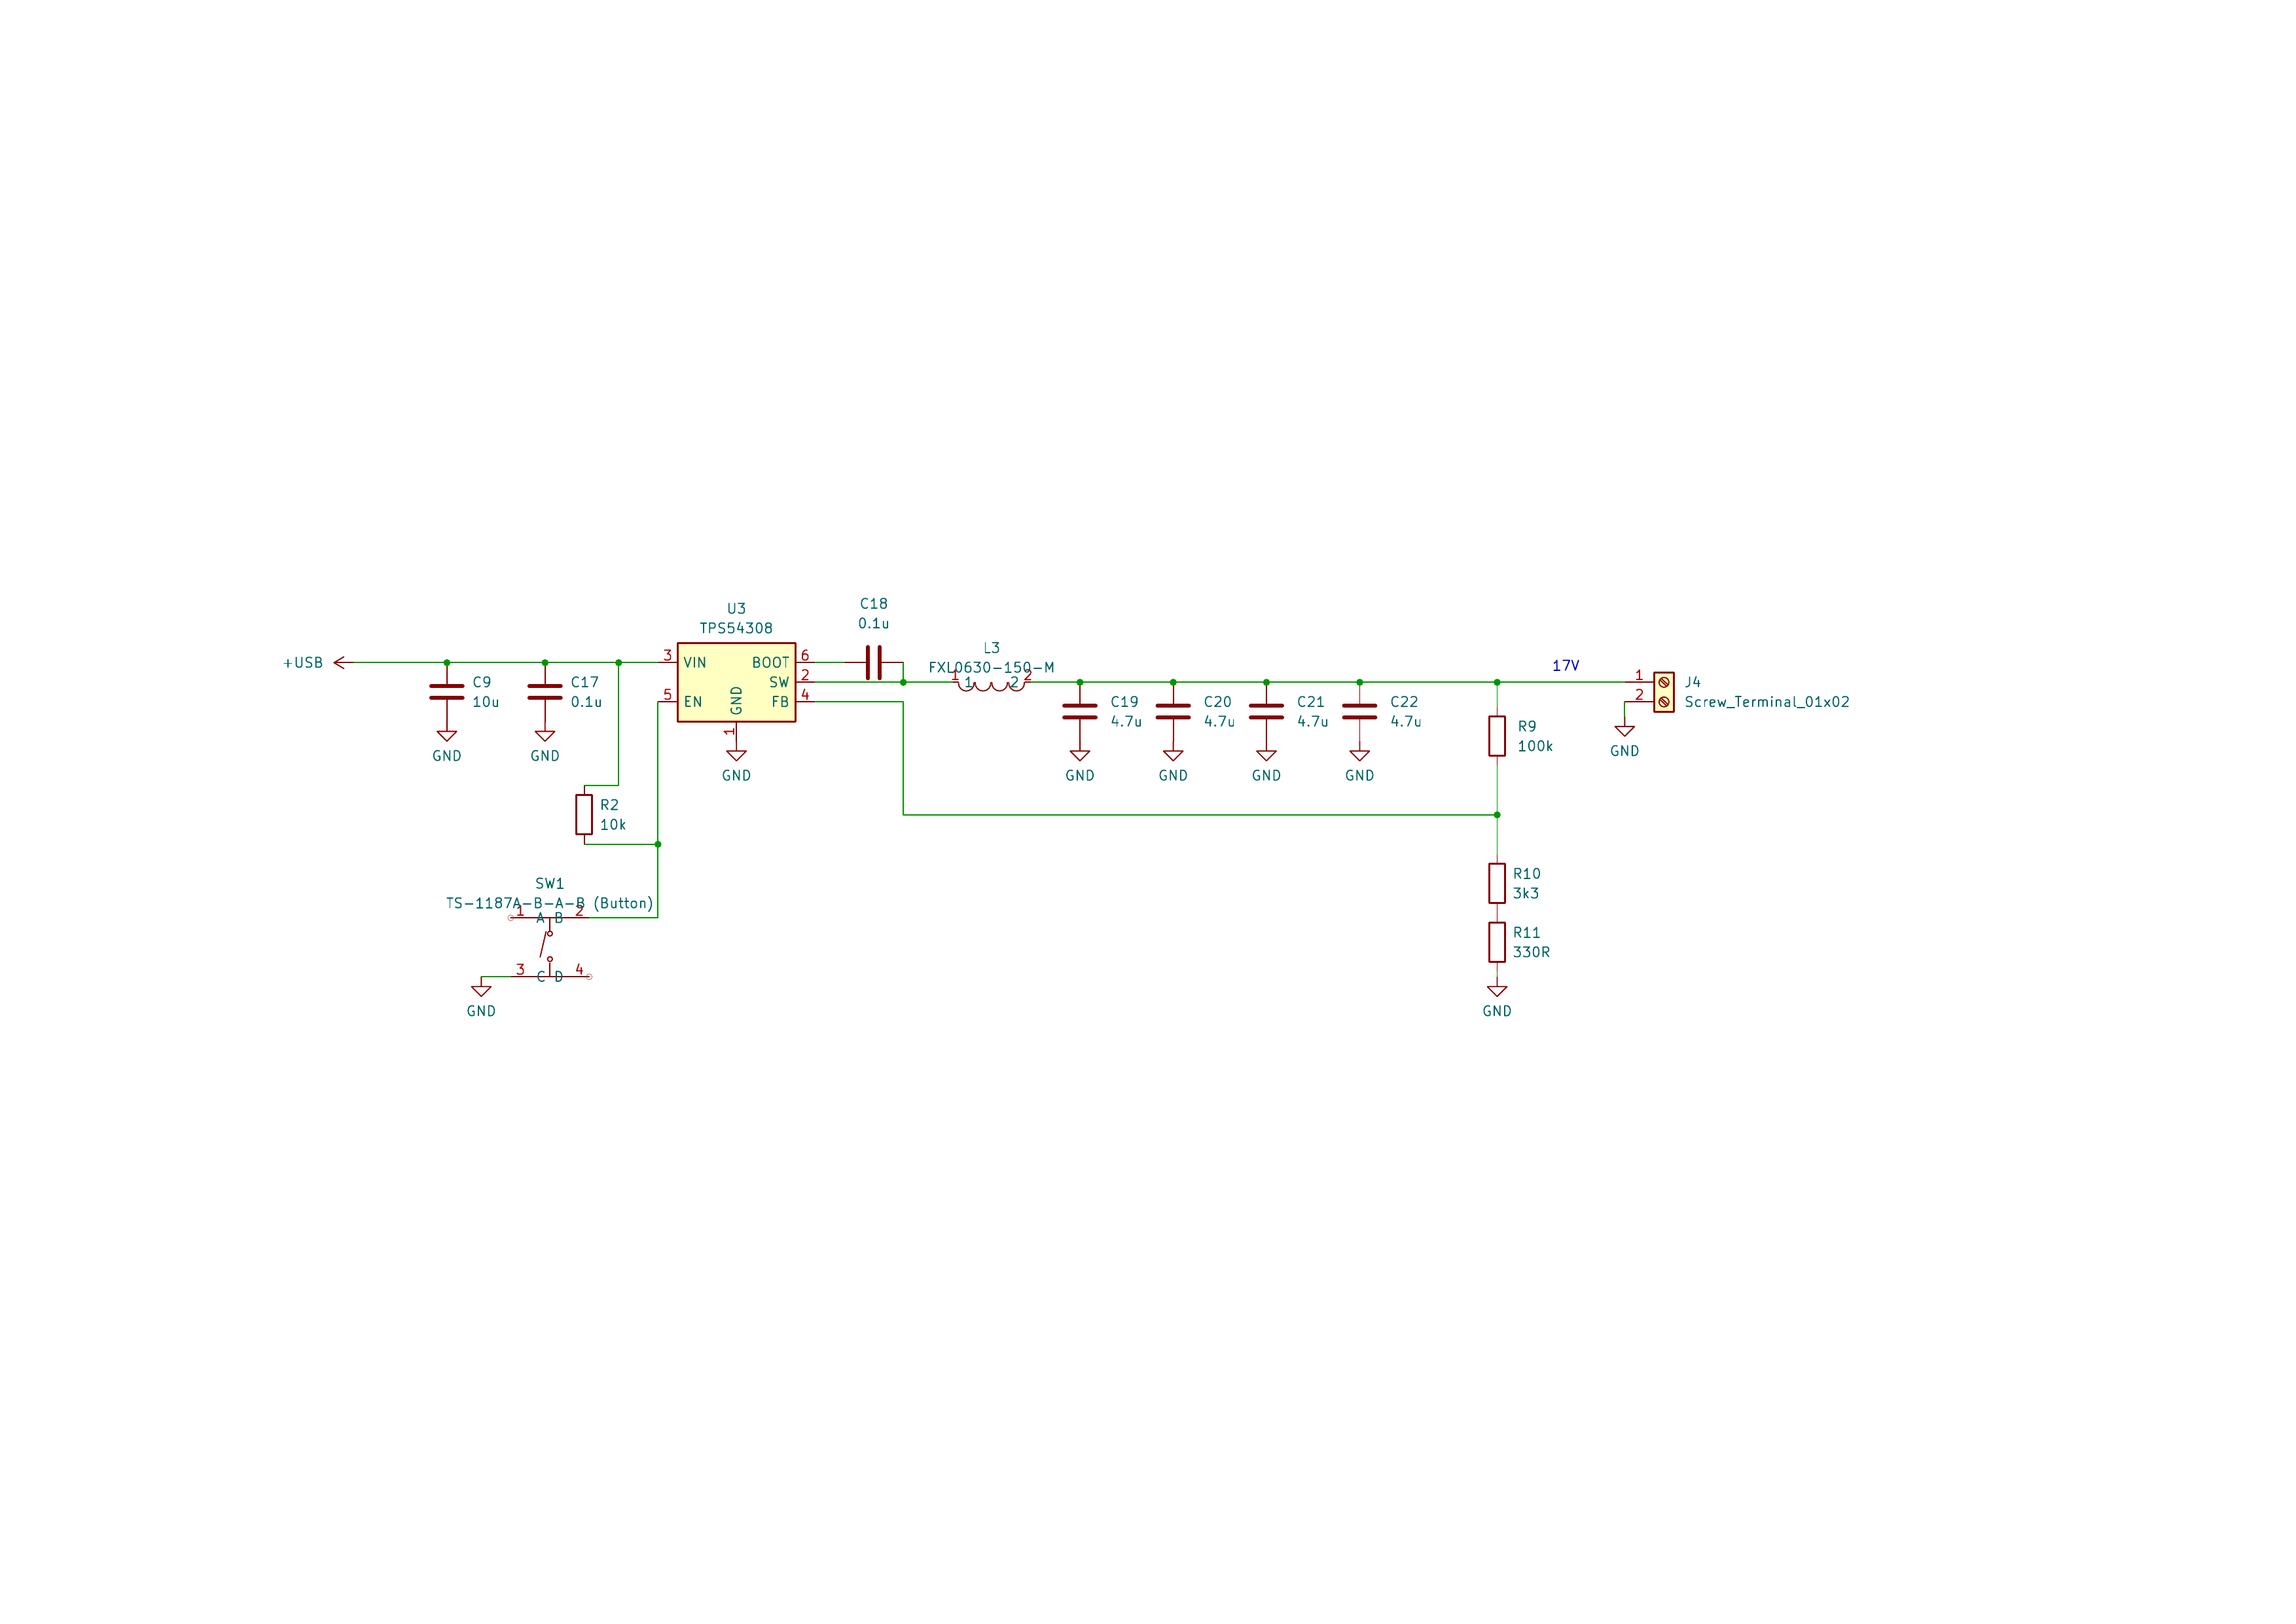
\includegraphics[width=0.95\textwidth]{schematics-3.png}
  \caption{Jetson power regulator schematic (Sheet 3 of 4).}
  \label{fig:schematic-full-3}
\end{figure}

\begin{figure}[H]
  \centering
  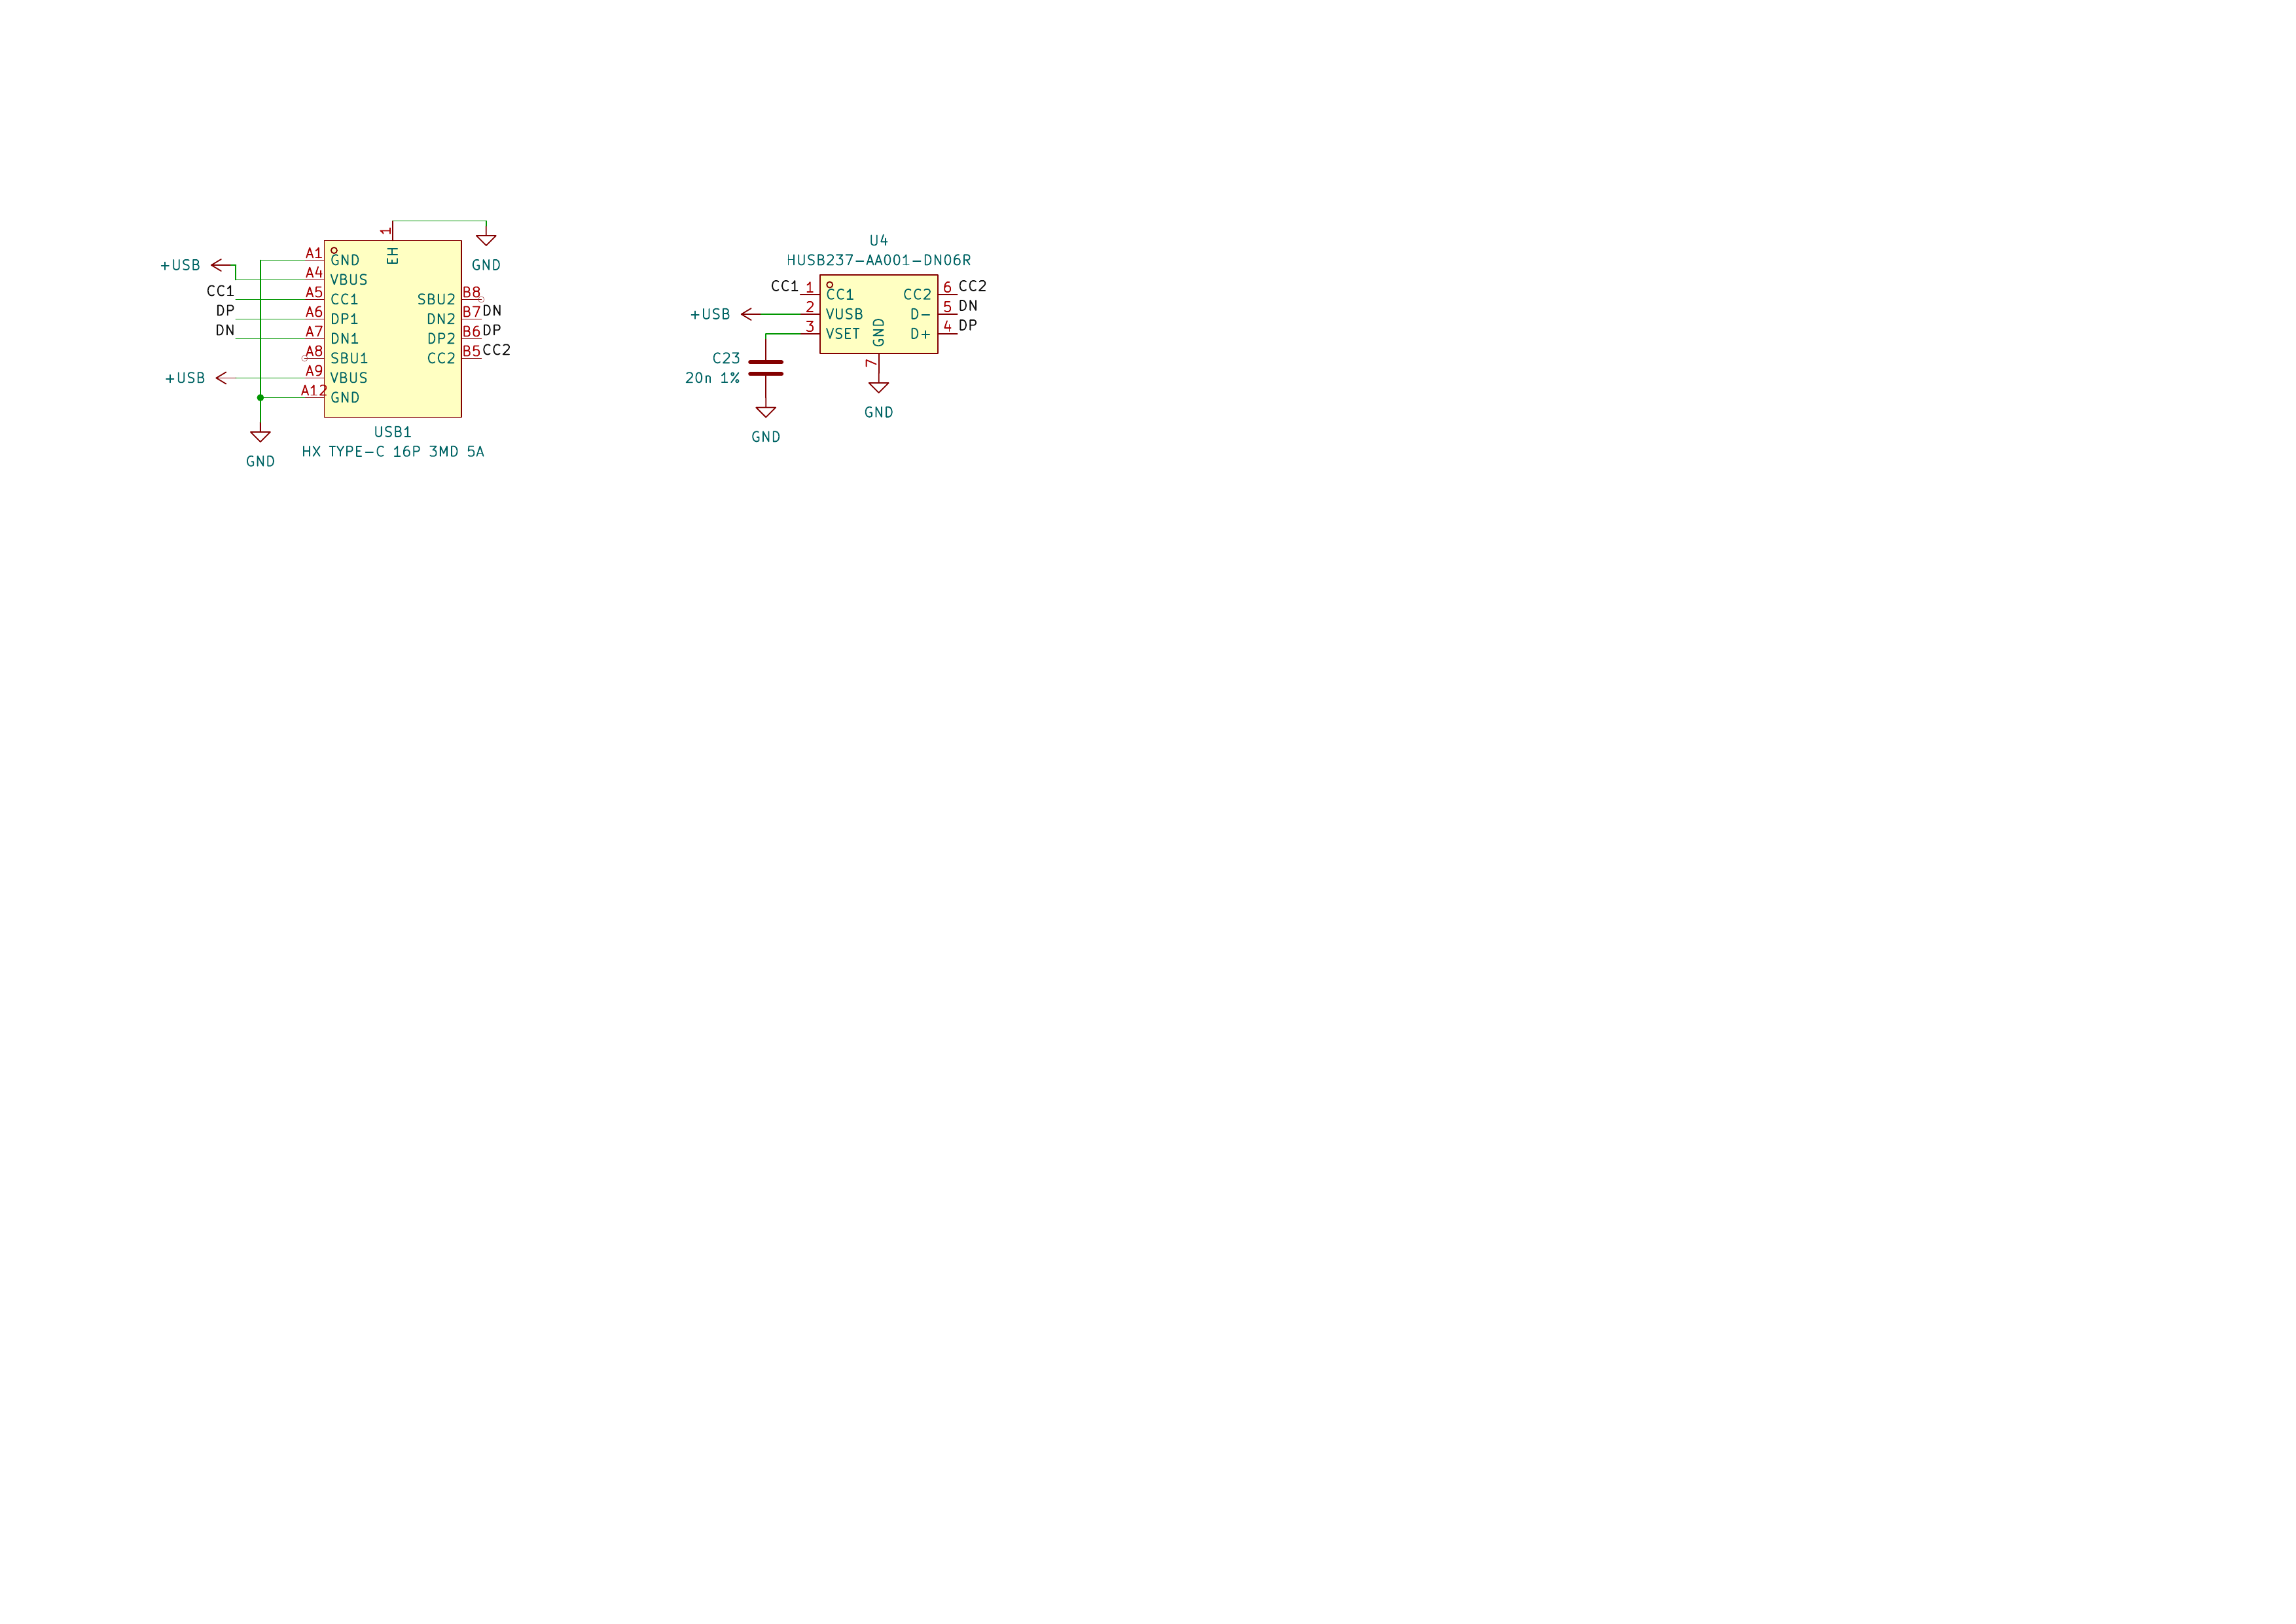
\includegraphics[width=0.95\textwidth]{schematics-4.png}
  \caption{USB-C connector and PD controller schematic (Sheet 4 of 4).}
  \label{fig:schematic-full-4}
\end{figure}

\section{Bill of Materials}
\label{app:bom}

Table~\ref{tab:bom} lists the key components for the PCB assembly.

\begin{table}[H]
  \centering
  \caption{Bill of Materials for Tracking Cam Prototype 0.5.}
  \label{tab:bom}
  \small
  \begin{tabular}{@{}clcc@{}}
    \toprule
    \textbf{Ref} & \textbf{Description} & \textbf{Qty} & \textbf{Value/Part} \\
    \midrule
    U2, U3      & Buck converter, 3A, SOT-23-6  & 3  & TPS54308DDCT \\
    U4          & USB PD sink controller, DFN-6 & 1  & HUSB237-AA001-DN06R \\
    U9          & MCU, ARM Cortex-M4, LQFP-64   & 1  & STM32F405RGT6 \\
    L1, L2, L3  & Power inductor, 15$\mu$H     & 3  & FXL0630-15q-M \\
    X7          & Crystal, 8MHz, SMD            & 1  & X322516MLB4SI \\
    USB1        & USB-C receptacle, 16P, 5A     & 1  & HX TYPE-C 16P \\
    J1          & Header, 6-pin, 2.54mm         & 1  & Samtec ESQ-106-33-L-D \\
    J4          & Screw terminal, 2-pin         & 1  & Screw\_Terminal\_L01x02 \\
    SW1         & Tactile switch, SMD           & 1  & TS-1187A-B-A-B \\
    D1, D3      & LED, SMD 0603                 & 2  & Green/Red \\
    C98-C108    & Capacitor, ceramic, 100nF     & 5  & 100nF, 50V \\
    C101        & Capacitor, ceramic, 4.7$\mu$F  & 1  & 4.7$\mu$F, 16V \\
    C126, C103  & Capacitor, ceramic, 2.2$\mu$F & 2  & 2.2$\mu$F, 16V \\
    C99, C100   & Capacitor, ceramic, 10pF      & 2  & 10pF, 50V \\
    C23         & Capacitor, ceramic, 20nF      & 1  & 20nF, 1\% \\
    \bottomrule
  \end{tabular}
\end{table}

Note: Additional passive components (resistors, capacitors) for the
regulator circuits are not listed exhaustively. See schematics for
complete component values.

\end{document}
